\chapter{Model Interpretation and Visualisation}
\label{chap:Model Interpretation and Visualisation}

This chapter delves into the interpretability of our models, offering insights into the decision-making processes of the neural networks. By visualizing model filters, feature maps, and utilizing techniques such as PCA and t-SNE, we aim to elucidate how different models perceive and classify plant disease images. Furthermore, we explore advanced interpretability methods, including saliency maps and nearest neighbor analysis, to provide a comprehensive understanding of the underlying mechanisms driving model predictions. Through these analyses, we aim to not only compare the effectiveness of different models but also enhance the transparency and explainability of our best-performing model (VGG16 Base Model).
\par\vspace{1em}

\begin{enumerate}
  \item Visualizing CNN Layers - Techniques for Visualization (Filter, Feature Maps)
  \item Visualizing features map with a masked image and a normal one
  \item Visualizing features map of images of different classes
  \item Other Model Interpretation Techniques - PCA, T-SNE, Nearest Neighbors, Saliency Maps
\end{enumerate}

\par\vspace{1em}

\section{Model Interpretation}

Model interpretation at heart, is to find out ways to understand model decision making policies better. This is to enable fairness, accountability and transparency which will give humans enough confidence to use these models in real-world problems which a lot of impact to business and society. Hence, there are techniques which have existed for a long time now, which can be used to understand and interpret models in a better way. These can be grouped under the following two major categories.

\begin{enumerate}
    \item Exploratory analysis and visualization techniques like clustering and dimensionality reduction.
    \item Model performance evaluation metrics like precision, recall, accuracy, ROC curve and the AUC (for classification models) and the coefficient of determination (R-square), root mean-square error, mean absolute error (for regression models).
\end{enumerate}

In our research, we'll be focussing more on visualisation part such as visualising feature space using dimensionality reduction technique, feature map visualisation, etc.  \par\vspace{1em}

Model Interpretation is very important to reduce biases in our training data. For Example: in saliency map fig \ref{fig:smap-1}, we are using a dog breed classifier to predict the dog classes but the model instead of focusing on the dog features to classify wolf or not, it actually focus on the background of the picture and predict wolf if the background contain snow and not-wolf if no snow is present. So, using appropriate model interpretation techniques (here, using a saliency map) we can find such biases in our model and get a glimpse of how the model is making the predictions without taking our model as a complete black box.\par\vspace{1em}


\begin{figure}
    \centering
    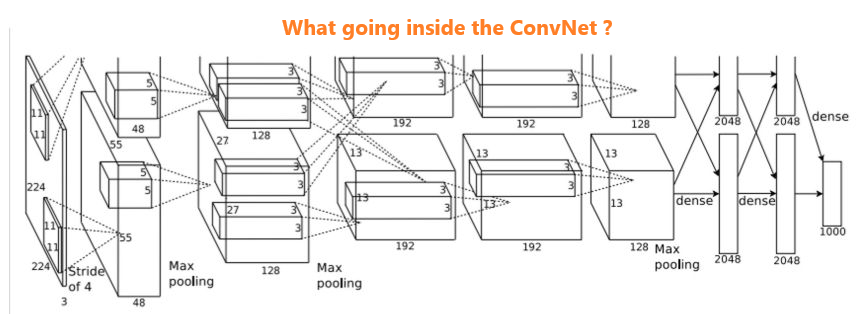
\includegraphics[width=\linewidth]{graphics/chapter6/model interpretation.png}
    \caption{Importance of Model Interpretation}
    \label{fig:model-interpretationj}
\end{figure}

\subsection{Understanding Machine Learning Model Interpretation}
    Machine Learning has seen widespread industry adoption only in the last couple of years. Hence, model interpretation as a concept is still mostly theoretical and subjective. Any machine learning model at its heart has a response function which tries to map and explain relationships and patterns between the independent (input) variables and the dependent (target or response) variable(s). \par\vspace{1em}

    When a model predicts or finds our insights, it takes certain decisions and choices. Model interpretation tries to understand and explain these decisions taken by the response function i.e., the what, why and how. The key to model interpretation is transparency, the ability to question, and the ease of understanding model decisions by humans. The three most important aspects of model interpretation are explained as follows.

    \begin{enumerate}
        \item What drives model predictions? We should have the ability to query our model and find out latent feature interactions to get an idea of which features might be important in the decision-making policies of the model. This ensures fairness of the model.
        \item Why did the model take a certain decision? We should also be able to validate and justify why certain key features were responsible in driving certain decisions taken by a model during predictions. This ensures accountability and reliability of the model.
        \item How can we trust model predictions? We should be able to evaluate and validate any data point and how a model takes decisions on it. This should be demonstrable and easy to understand for key stakeholders that the model works as expected. This ensures transparency of the model.
    \end{enumerate}
    
Interpretability also popularly known as human-interpretable interpretations (HII) of a machine learning model is the extent to which a human (including non-experts in machine learning) can understand the choices taken by models in their decision-making process (the how, why and what).\par\vspace{1em}

When comparing models, besides model performance, a model is said to have a better interpretability than another model if its decisions are easier to understand by a human than the decisions from the other model.\cite{WEBSITE:model-interpretation-medium}

\subsection{The Importance of Machine Learning Model Interpretation}
    When tackling machine learning problems, data scientists often have a tendency to fixate on model performance metrics like accuracy, precision and recall and so on (This is important no doubt!). This is also prevalent in most online competitions around data science and machine learning. However, metrics only tell a part of the story of a model’s predictive decisions. Over time, the performance might change due to model concept drift caused by various factors in the environment. Hence, it is of paramount importance to understand what drives a model to take certain decisions.\par\vspace{1em}

    Some of us might argue if a model is working great why bother digging deeper? Always remember that when solving problems in the real-world, for the business to trust your model predictions and decisions, they will keep asking the question, “Why should I trust your model?” and this makes perfect sense. Would you be satisfied with a model just predicting and taking decisions (the what) like if a person has cancer or diabetes, if a person might be a risk to society or even if a customer will churn? Maybe not, we might prefer it more if we could know more about the model’s decision process (the why and how). This gives us more transparency into why the model makes certain decisions, what might go wrong in certain scenarios and over time it helps us build a certain amount of trust on these machine learning models.\cite{WEBSITE:model-interpretation-medium}\par\vspace{1em}


\section{Visualising First Layer Filters}

In this section, we perform visualization of the first layer filter learned by the VGG16 base model and CNN10L model.The first layer filters are critical as they capture basic features such as edges, textures, and colors, which are foundational for subsequent layers.\par\vspace{1em}

\begin{figure}
    \centering
    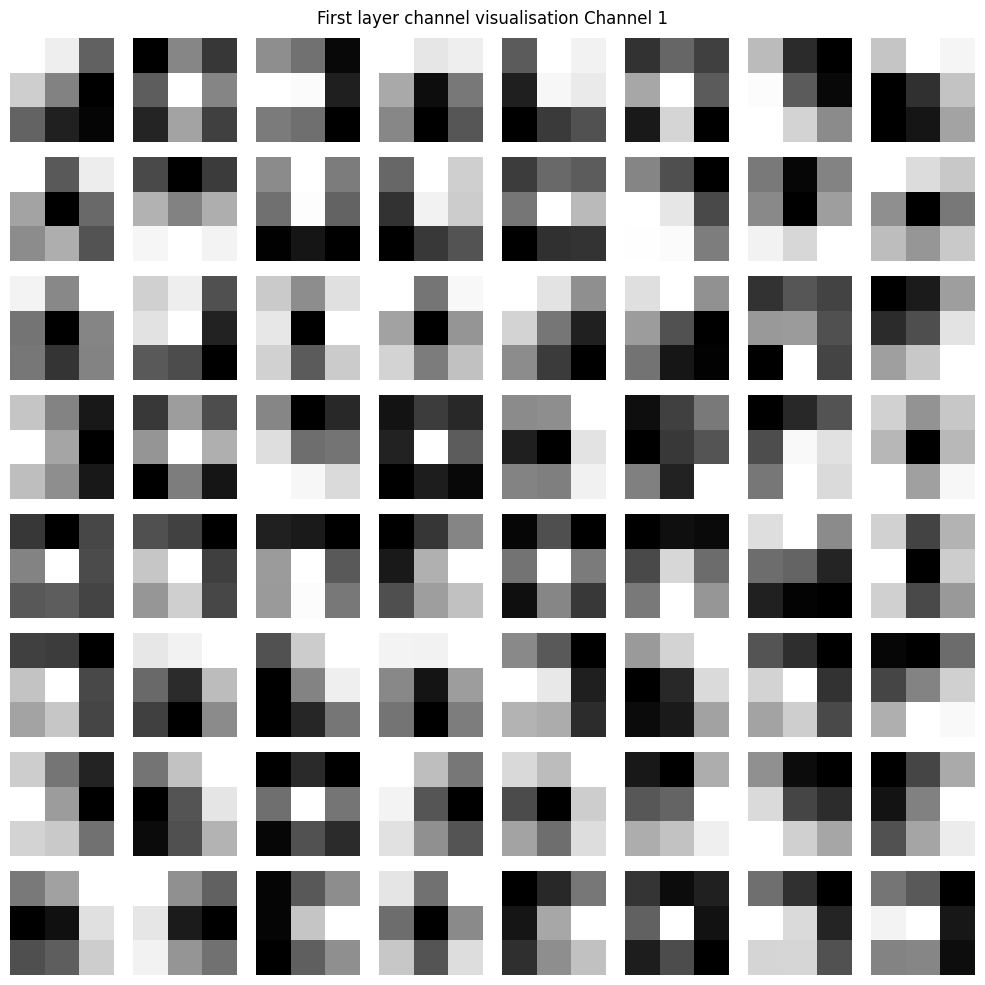
\includegraphics[width=1\linewidth]{graphics//chapter7/vgg16 first filter.png}
    \caption{VGG16 First Layer First 64 Filters}
    \label{fig:vgg-filter}
\end{figure}

\begin{figure}
    \centering
    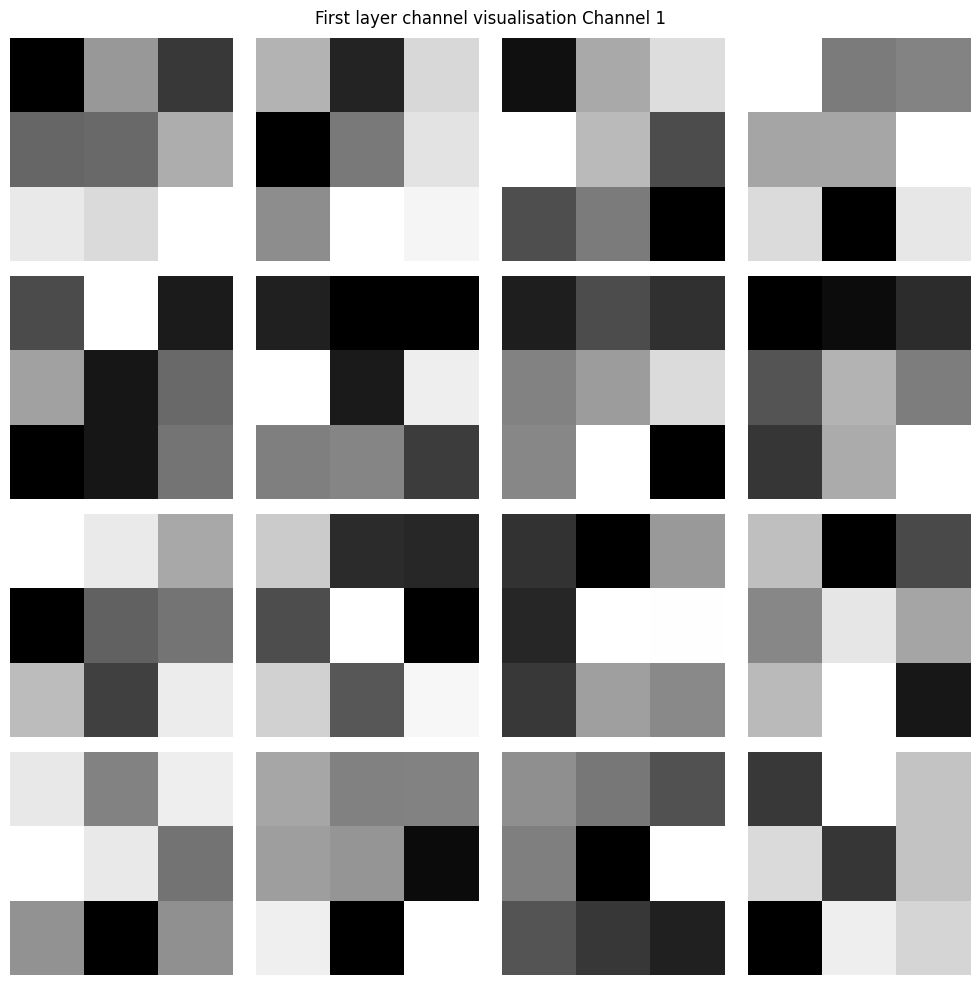
\includegraphics[width=1\linewidth]{graphics//chapter7/CNN10L filter.png}
    \caption{CNN10L First Layer 16 Filters}
    \label{fig:cnn10l-filter}
\end{figure}

\textbf{Observations of Fine Tune VGG16 Base Model Filter: }

\begin{itemize}
    \item \textbf{Edge and Texture Detection:}\\
    The first layer filters of the fine-tuned VGG16 model prominently detect edges and basic textures. The filters are well-defined, showing a variety of orientations and frequencies, which are essential for capturing the structure of the input images.\\
    The filters are appear to be less diverge as compare to each other, most of them seems to have the same structure but differ in their orientation, flip, rotate or are complete opposite of each other.\\
    For eg: in fig: \ref{fig:vgg-filter} filter of row-6 and col-5; and filter of row-8 and col-8 are same. Similarly, for filter of (4-row, 4-col) and of (8, 6); (8, 1) and (8, 2) seems to have the same structure but differ in their orientation. Filter of (1, 1), (3, 8) and (6, 8) also have similar structure but have different orientation, many such filters can be pick out from the figure \ref{fig:vgg-filter}\\
    These foundational features contribute to the model’s ability to accurately classify different diseases by building on these basic patterns in deeper layers.
\end{itemize}

\textbf{Observations of Fine Tune CNN10L Model Filter: }
\begin{itemize}
    \item \textbf{Edge and Basic Pattern Detection:}\\
    Similar to VGG16, the first layer filters of the CNN10L model also detect edges, lines, textures, gradients and basic patterns. However, the filters appear more diverse and slightly less defined compared to those of the fine-tuned VGG16 model.\\
    The filters show a wide range of structure but may not capture as wide a variety of textures and colors as effectively as by VGG16 model.\\
    From the fig: \ref{fig:cnn10l-filter}, we observe that filter in (3, 3) and in fig: \ref{fig:vgg-filter}, filter in (2, 3) seems to have similar structure but differ in their orientation.\\
    
    \item \textbf{Specialization:}\\
    Due to small number of filters present in the first layer and since it is trained only on Plant village datasets, the filter are less structured and specialised on the plant village datasets, so, they'll have low generalisation capability compare to vgg models.
    The filters of the CNN10L model are somewhat specialized to the specific characteristics of the Plant Village dataset so, even though they do capture basic patterns, their diverse nature of filter suggests that the model might rely more on specific patterns present in the training data, which can limit generalization compared to VGG16.
\end{itemize}

\section{Features Map Visualisation}

\subsection{Feature Map Visualisation of Apple Black Rot}
\begin{figure}
    \centering
    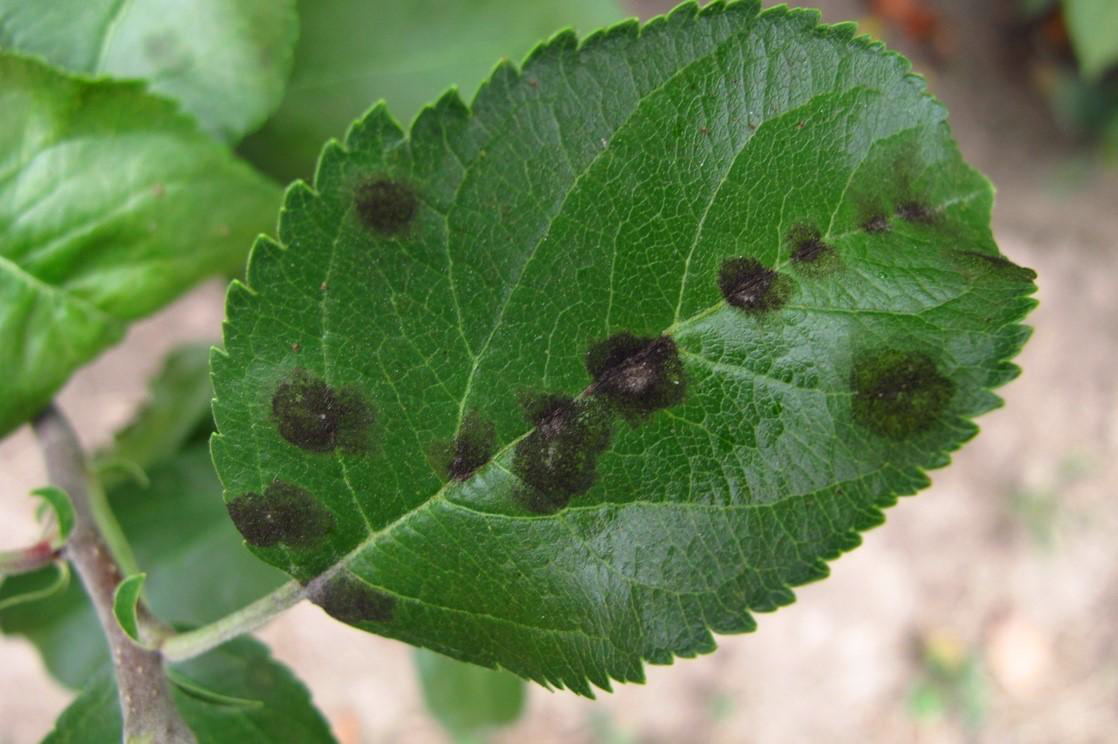
\includegraphics[width=0.5\linewidth]{graphics//chapter7/apple black rot.png}
    \caption{Apple Scab}
    \label{fig:apple-black-rot}
\end{figure}

To interpret the feature extraction process at different depths of the fine-tuned VGG16 model, we visualized the feature maps at layers 2, 5, 9, 13, and 17. These layers represent increasing levels of abstraction, from basic edge detection to complex pattern recognition.\par\vspace{1em}

\begin{figure}
    \centering
    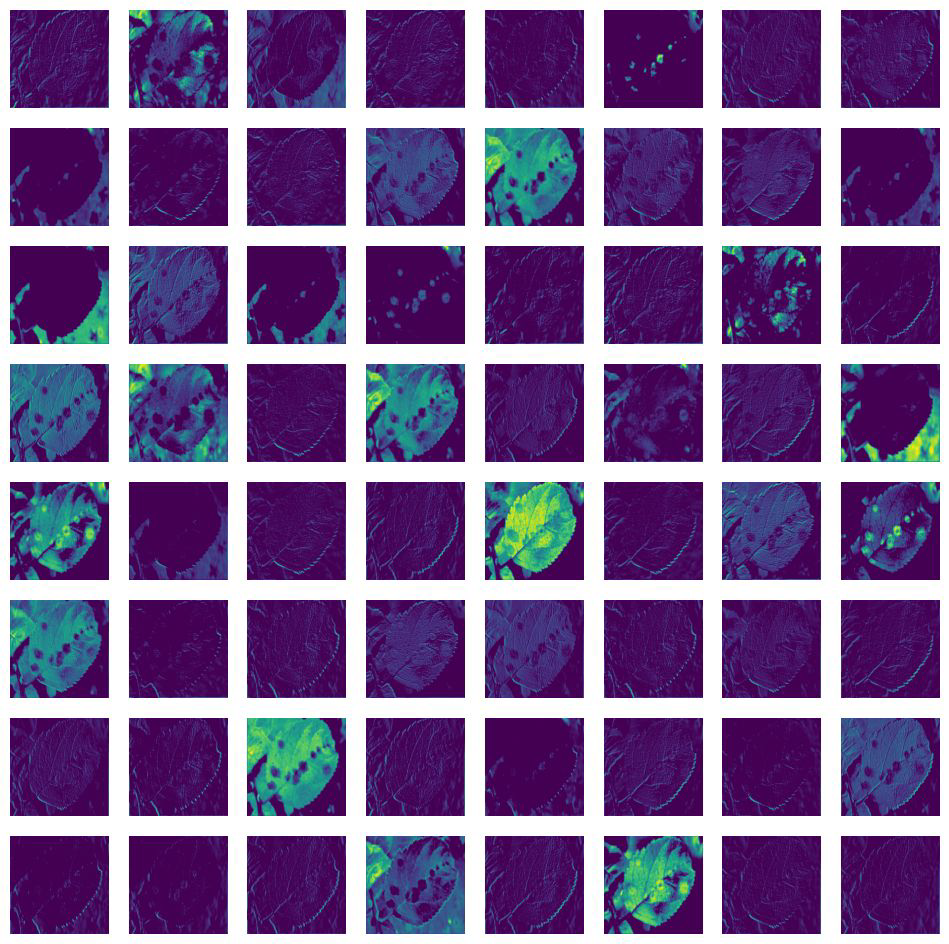
\includegraphics[width=0.75\linewidth]{graphics//chapter7/apple black rot fmap1.png}
    \caption{Feature Map of Apple Scab in Layer 2 produced by fine-tuned VGG16 base model}
    \label{fig:abr-fmap1}
\end{figure}

\begin{figure}
    \centering
    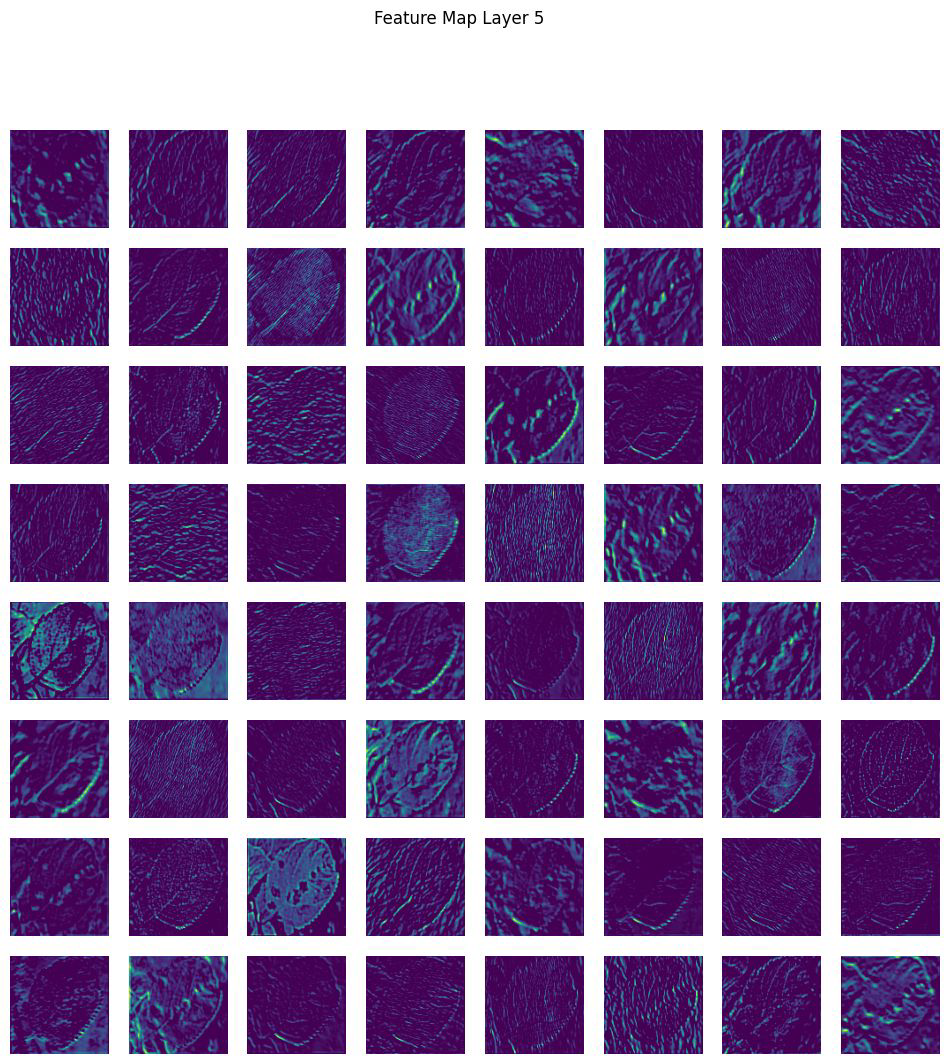
\includegraphics[width=\linewidth]{graphics//chapter7/abr fmap layer5.png}
    \caption{Feature Map of Apple Scab in Layer 5 produced by fine-tuned VGG16 base model}
    \label{fig:abr-fmap2}
\end{figure}

\begin{figure}
    \centering
    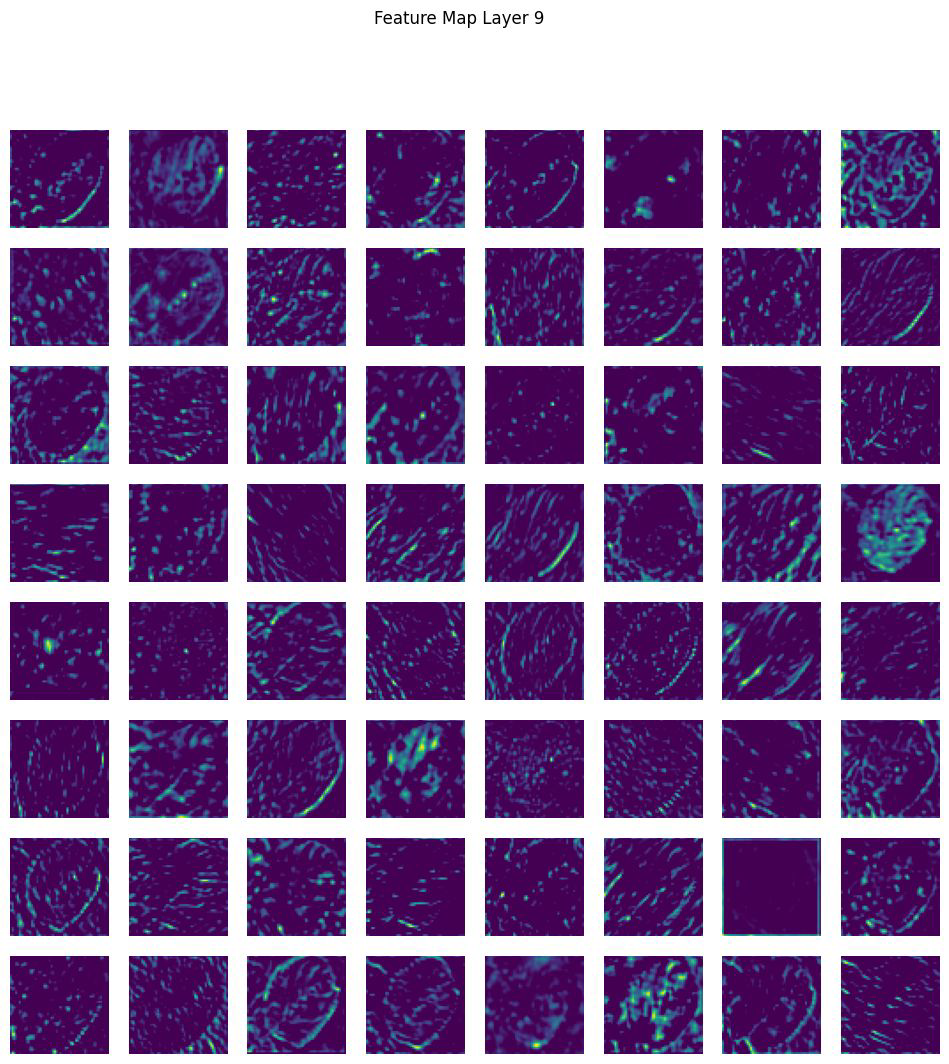
\includegraphics[width=\linewidth]{graphics//chapter7/abr feature map layer 9.png}
    \caption{Feature Map of Apple Scab in Layer 9 produced by fine-tuned VGG16 base model}
    \label{fig:abr-fmap3}
\end{figure}

\begin{figure}
    \centering
    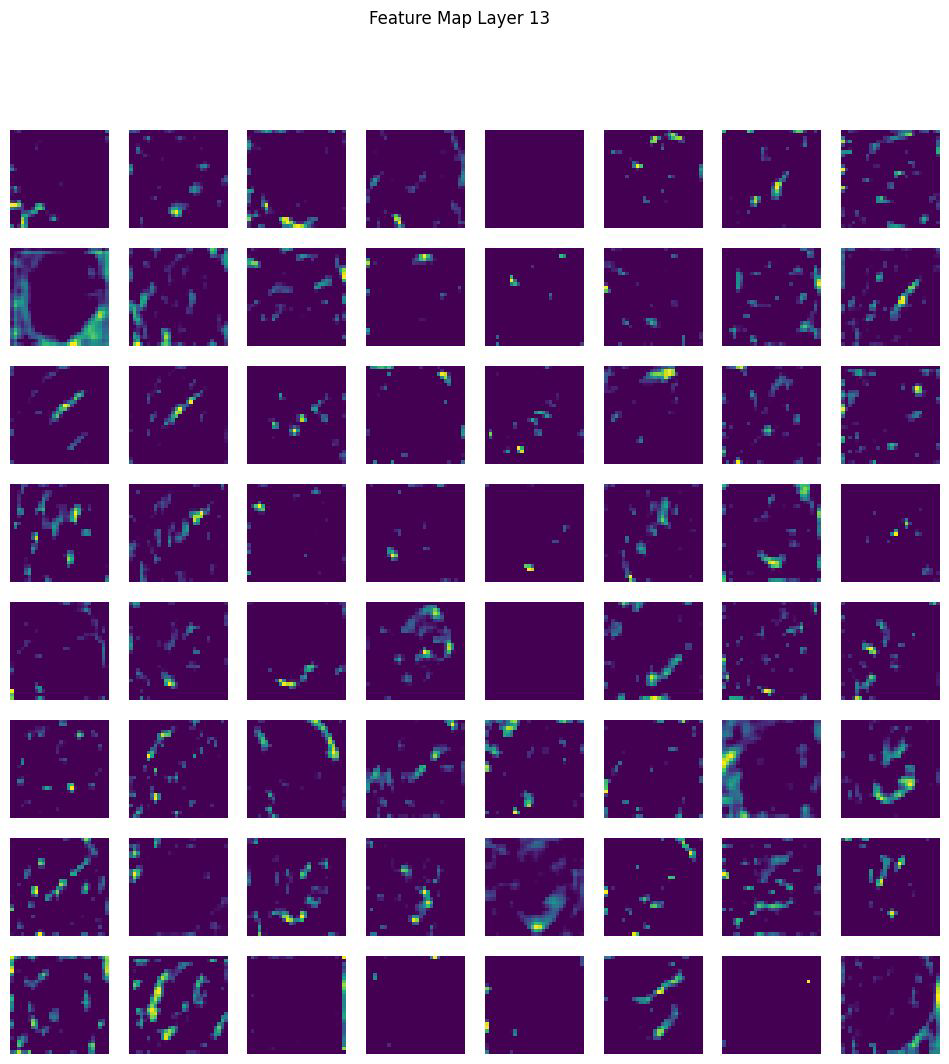
\includegraphics[width=\linewidth]{graphics//chapter7/abr fmap 13.png}
    \caption{Feature Map of Apple Scab in Layer 13 produced by fine-tuned VGG16 base model}
    \label{fig:abr-fmap4}
\end{figure}

\begin{figure}
    \centering
    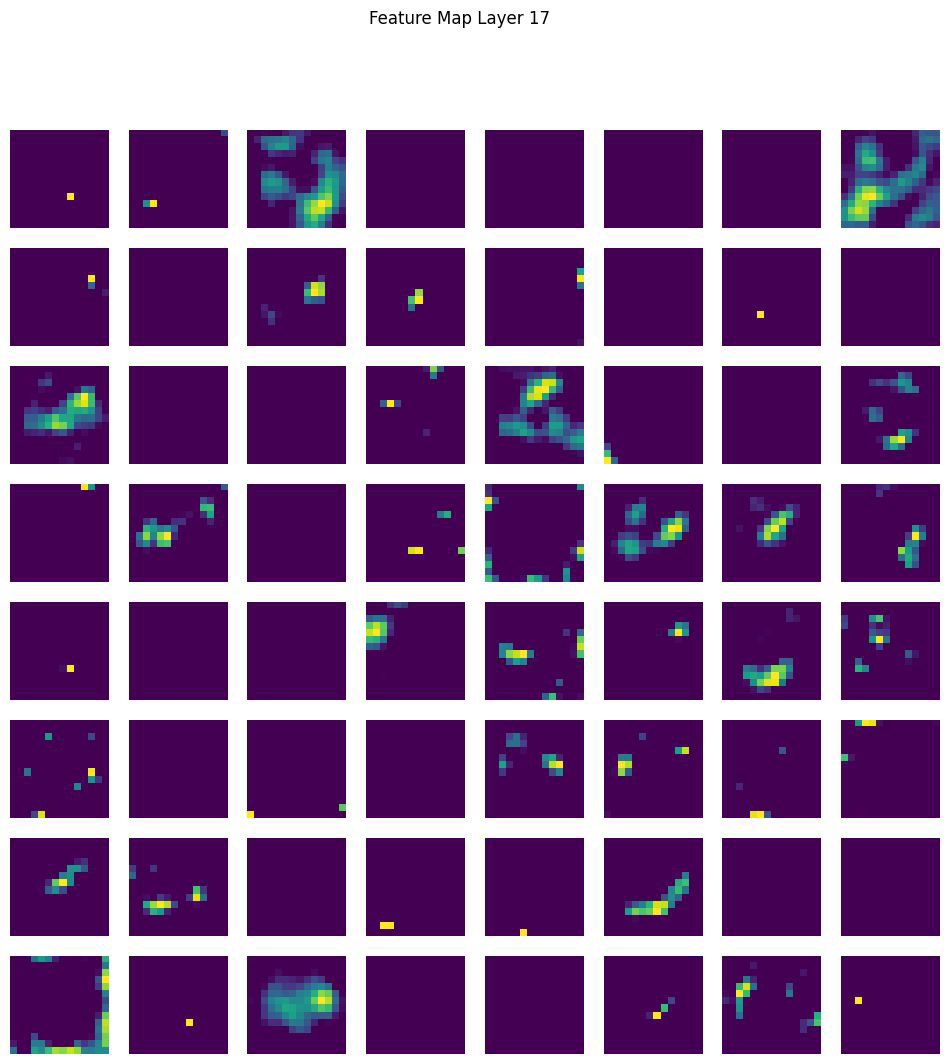
\includegraphics[width=1\linewidth]{graphics//chapter7/abr fmap 17.png}
    \caption{Feature Map of Apple Scab in Layer 17 produced by fine-tuned VGG16 base model}
    \label{fig:abr-fmap5}
\end{figure}


\textbf{Observation: }
\begin{itemize}
    \item \textbf{Layer2}\\
    \textbf{Basic Edge and Texture Detection:}
    The feature maps at this early layer primarily capture simple edges and textures. The activation patterns highlight basic structures in the input images, such as contours and edges of leaves. This layer serves as the foundation for more complex feature extraction in subsequent layers.
    \item \textbf{Layer5}\\
    \textbf{Enhanced Texture and Shape Recognition:}
    By layer 5, the feature maps show more complex textures and shapes. The model begins to detect patterns such as leaf veins and surface textures, which are more intricate than basic edges. These features are crucial for distinguishing between different types of diseases that affect the texture and surface appearance of leaves.
    \item \textbf{Layer9}\\
    \textbf{Intermediate Patterns and Details:}
    The feature maps at layer 9 capture intermediate patterns and details. The activations are more abstract, representing combinations of edges, textures, and shapes detected in earlier layers. This layer contributes to the model's ability to recognize more detailed and specific features of diseased leaves.
    \item \textbf{Layer13}\\
    \textbf{Complex Structures and Patterns:}
    At layer 13, the feature maps show complex structures and patterns, indicating a high level of abstraction. The activations capture specific disease characteristics such as spots, discolorations, and irregular shapes. This depth allows the model to differentiate between subtle differences in disease presentations.
    \item \textbf{Layer17}\\
    \textbf{High-Level Feature Integration:}
    The feature maps at layer 17 exhibit high-level feature integration. The activations represent very abstract and complex features that combine all previous layers' information. This layer is critical for final classification, as it integrates all detected patterns and structures to make a decision about the disease class.
\end{itemize}


\subsection{Feature Map Comparison of Apple Scab and Apple Black Rot}

In this section, to gain deeper insights into the feature extraction capabilities of our fine-tuned VGG16 model, we visualized and compared the feature maps for two distinct diseases: apple scab and apple black rot. This comparison aims to highlight how the model distinguishes between different disease characteristics at various layers. \par\vspace{1em}

\textbf{Observations: }\\
\begin{itemize}
    \item \textbf{Apple Scab:}\\
    The feature maps for apple scab reveal strong activations around the edges and surface spots characteristic of the disease. At intermediate layers, the model captures the distinct textures and discolorations typical of apple scab. In deeper layers, these features integrate to form a comprehensive representation, focusing on the scab's unique pattern and severity. This indicates that the model effectively learns to recognize the specific visual cues associated with apple scab, enabling precise classification.
    \item \textbf{Apple Black Rot:}\\
    For apple black rot, the feature maps show activations concentrated around the dark, rotted areas of the leaf. Early layers detect the edges of the rotted regions, while intermediate layers highlight the contrasting textures and colors associated with the rot. In the deepest layers, the model integrates these features to form a distinct representation of black rot, emphasizing the lesion's shape, color, and spread. This demonstrates the model's ability to capture and differentiate the unique visual signatures of black rot, ensuring accurate disease identification.
\end{itemize}


\begin{figure}
    \centering
    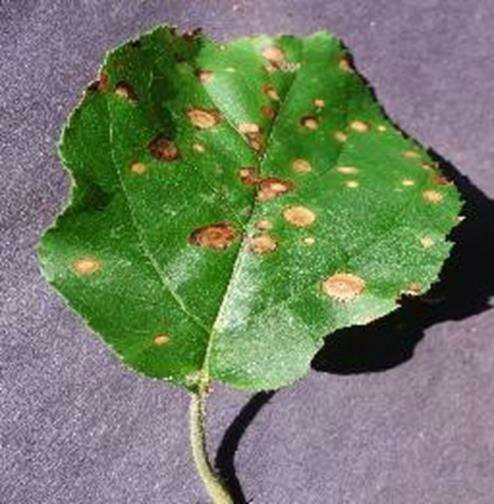
\includegraphics[width=0.5\linewidth]{graphics//chapter7/abr2.png}
    \caption{Apple Black Rot}
    \label{fig:abr-2}
\end{figure}

\begin{sidewaysfigure}
    \centering
    \begin{turn}{180}
        \begin{minipage}{\linewidth}
            \centering
            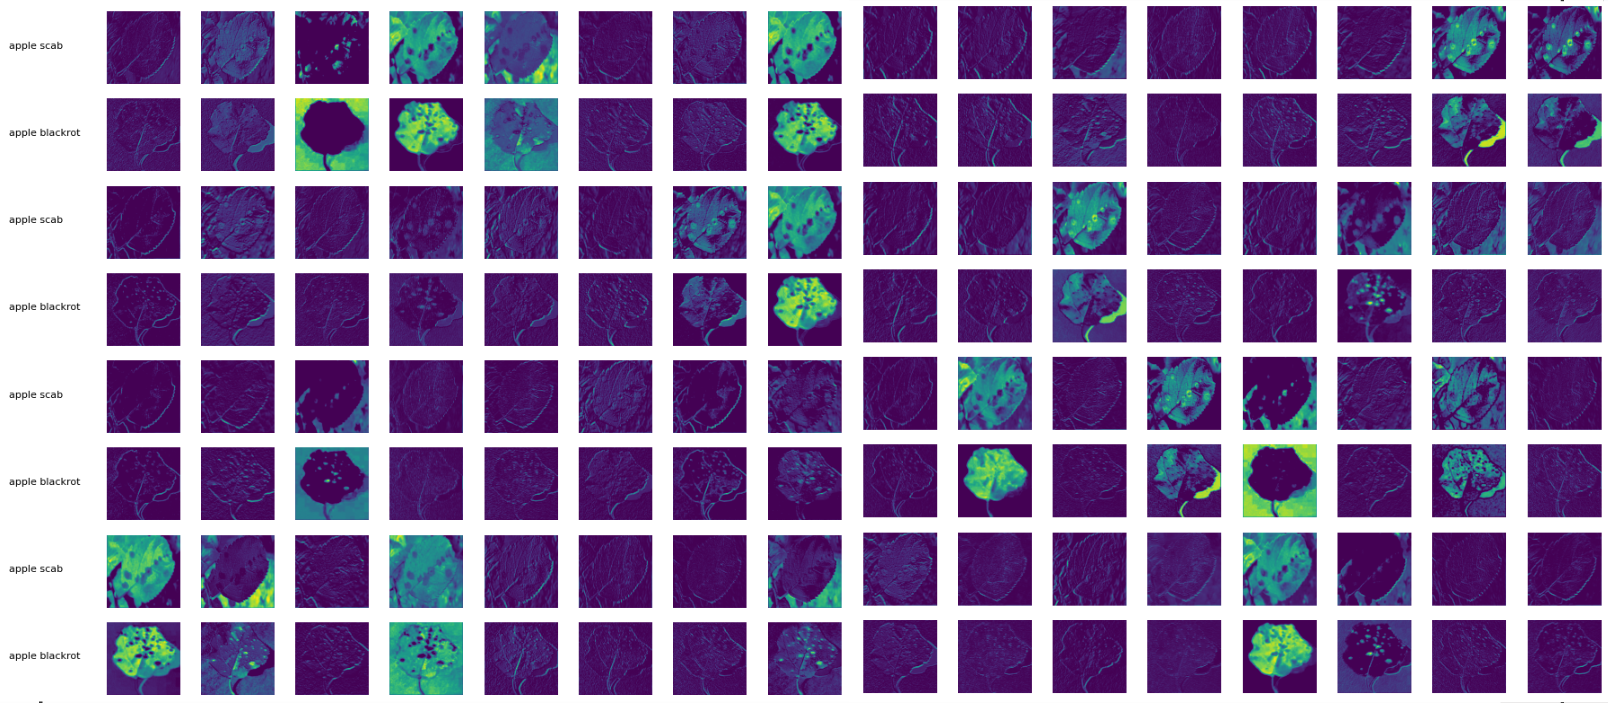
\includegraphics[width=1\linewidth]{graphics//chapter7/fmap comp as abr.png}
            \caption{VGG16 base model Layer-2, first 64 Feature Map Comparison with Apple Scab and Apple Black Rot image}
            \label{fig:comp-1}
        \end{minipage}
    \end{turn}
\end{sidewaysfigure}


\begin{sidewaysfigure}
    \centering
    \begin{turn}{180}
        \begin{minipage}{\linewidth}
        \centering
        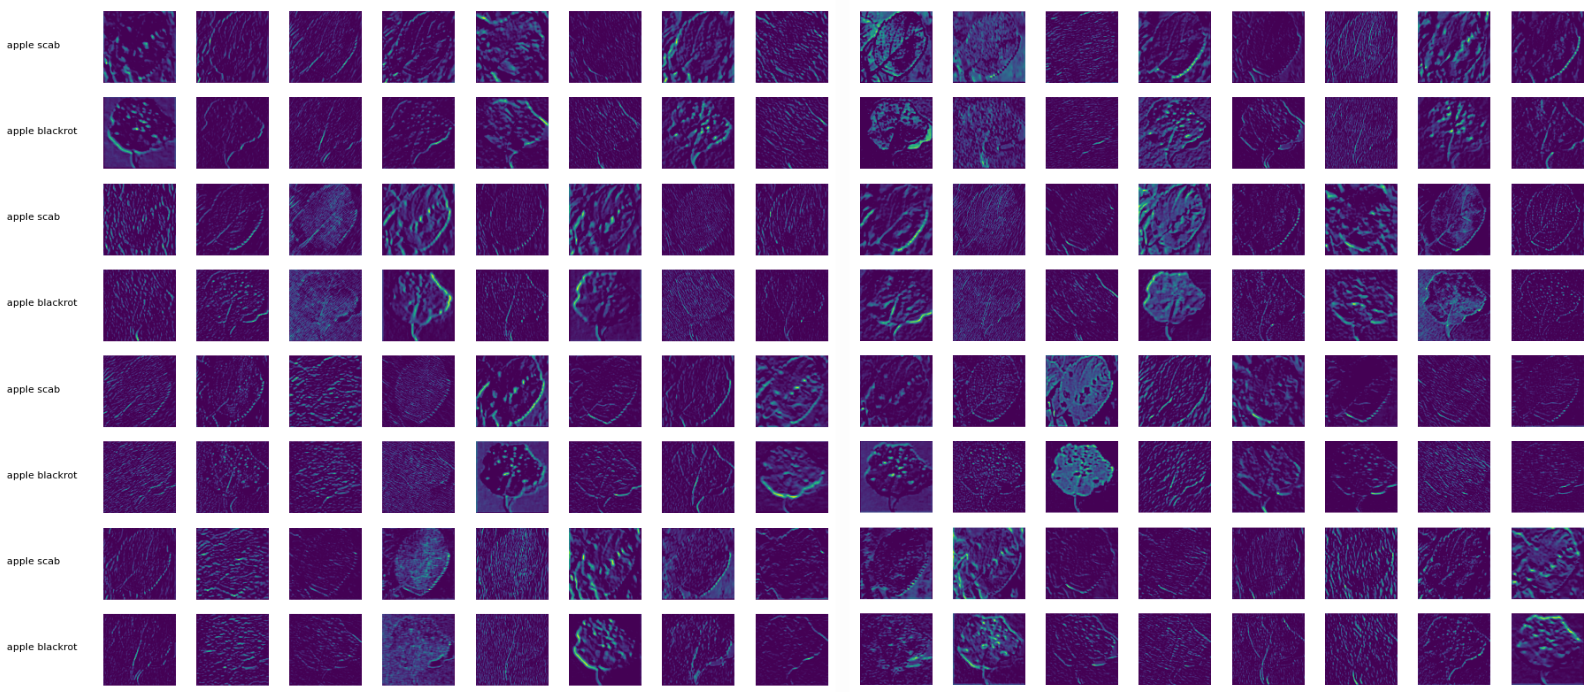
\includegraphics[width=1\linewidth]{graphics//chapter7/fmap comp abr as l5.png}
        \caption{VGG16 base model Layer-5, first 64 Feature Map Comparison with Apple Scab and Apple Black Rot image}
        \label{fig:comp-2}
        \end{minipage}
    \end{turn}
\end{sidewaysfigure}


\begin{sidewaysfigure}
    \centering
    \begin{turn}{180}
        \begin{minipage}{\linewidth}
        \centering
        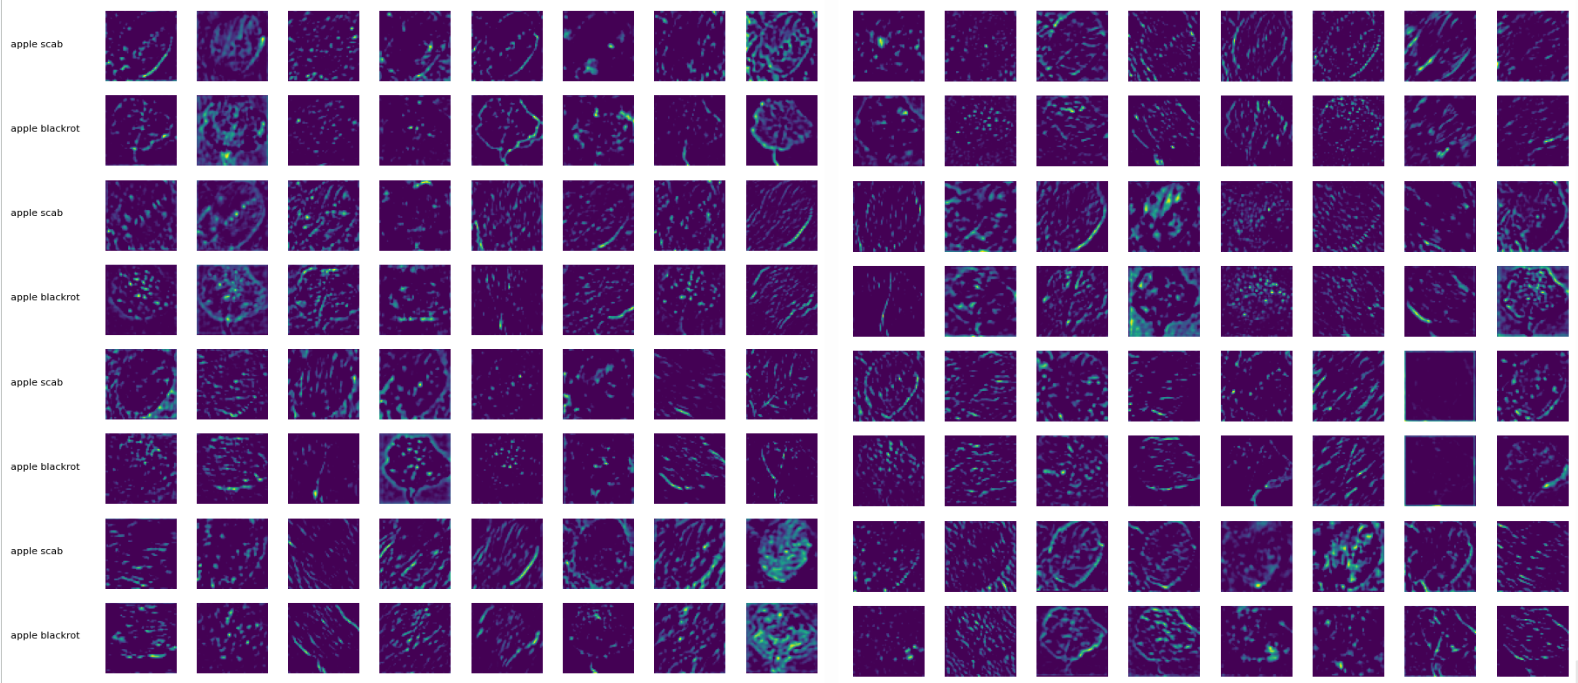
\includegraphics[width=1\linewidth]{graphics//chapter7/fmap comp abr as l9.png}
        \caption{VGG16 base model Layer-9, first 64 Feature Map Comparison with Apple Scab and Apple Black Rot image}
        \label{fig:comp-3}
        \end{minipage}
    \end{turn}
\end{sidewaysfigure}


\begin{sidewaysfigure}
    \centering
    \begin{turn}{180}
        \begin{minipage}{\linewidth}
        \centering
        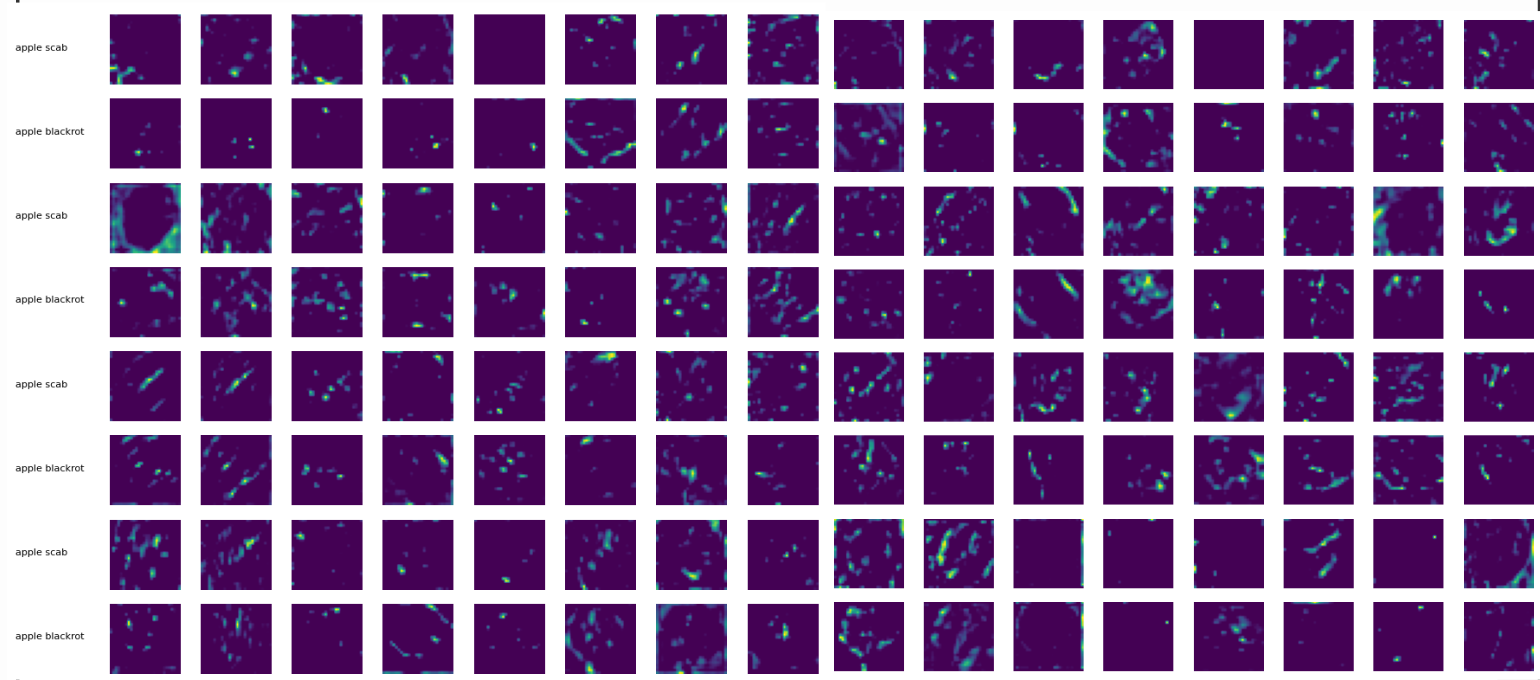
\includegraphics[width=1\linewidth]{graphics//chapter7/fmap comp l15 abr as.png}
        \caption{VGG16 base model Layer-13, first 64 Feature Map Comparison with Apple Scab and Apple Black Rot image}
        \label{fig:comp-4}
        \end{minipage}
    \end{turn}
\end{sidewaysfigure}

\begin{sidewaysfigure}
    \centering
    \begin{turn}{180}
        \begin{minipage}{\linewidth}
        \centering
        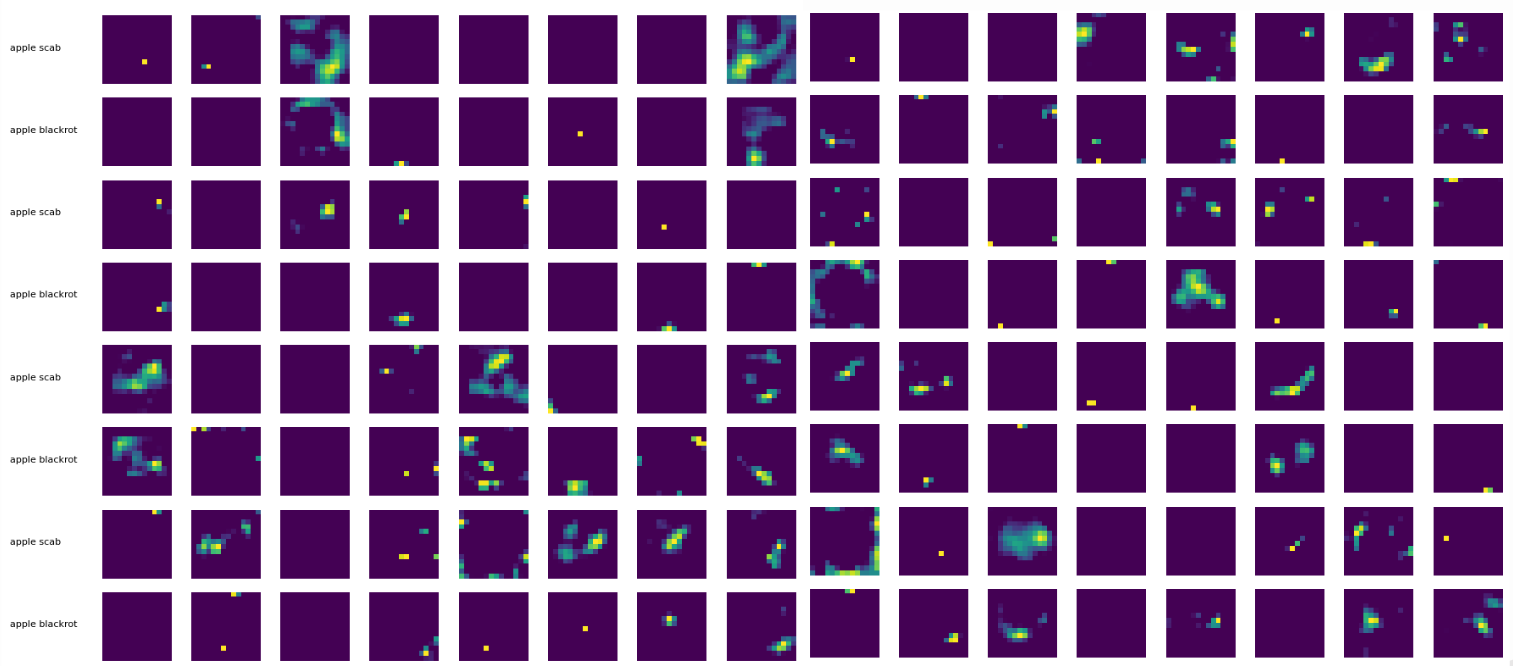
\includegraphics[width=1\linewidth]{graphics//chapter7/fmap comp abr as l17.png}
        \caption{VGG16 base model Layer-17, first 64 Feature Map Comparison with Apple Scab and Apple Black Rot image}
        \label{fig:comp-5}
        \end{minipage}
    \end{turn}
\end{sidewaysfigure}


\section{Feature Map comparison with Mask Image}
\begin{figure}
    \centering
    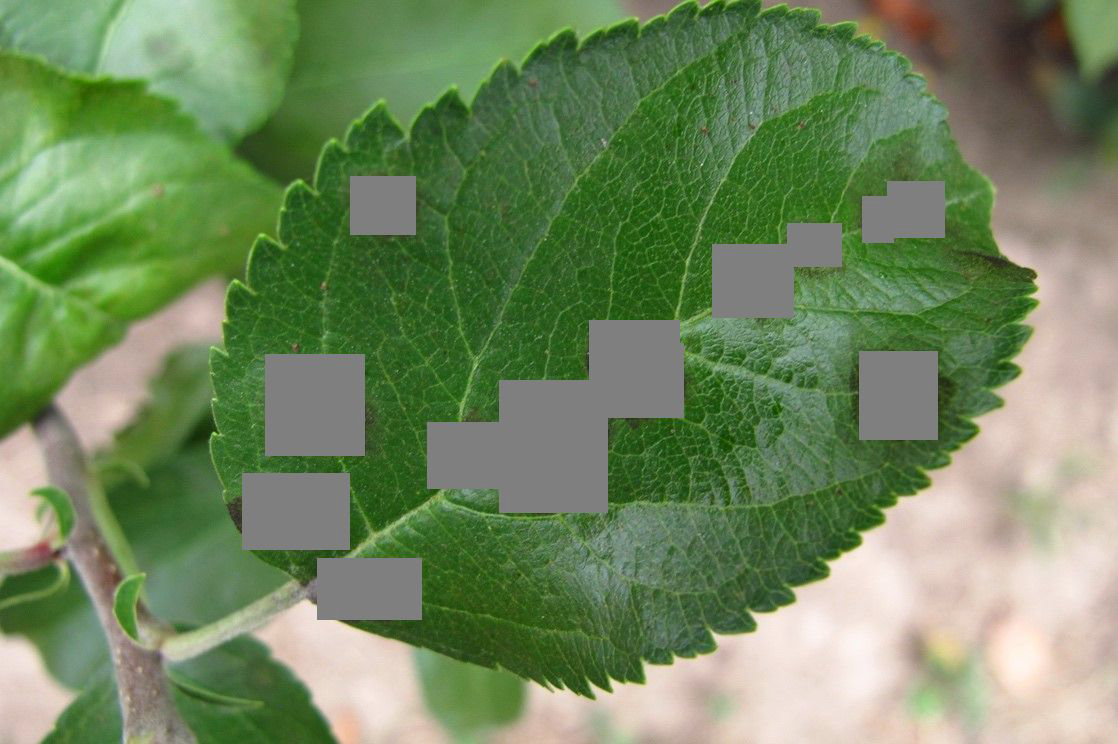
\includegraphics[width=0.5\linewidth]{graphics//chapter7/apple scab mask.png}
    \caption{Apple Scabs with Masks}
    \label{fig:apple-scab-mask}
\end{figure}

To further interpret the feature extraction capabilities of our fine-tuned VGG16 model, we visualized the feature maps using both a normal and a masked image. The masked image had a portion of the leaf covered with a grey mask to understand how the model handles occluded information.\par\vspace{1em}

\begin{sidewaysfigure}
    \centering
    \begin{turn}{180}
        \begin{minipage}{\linewidth}
        \centering
            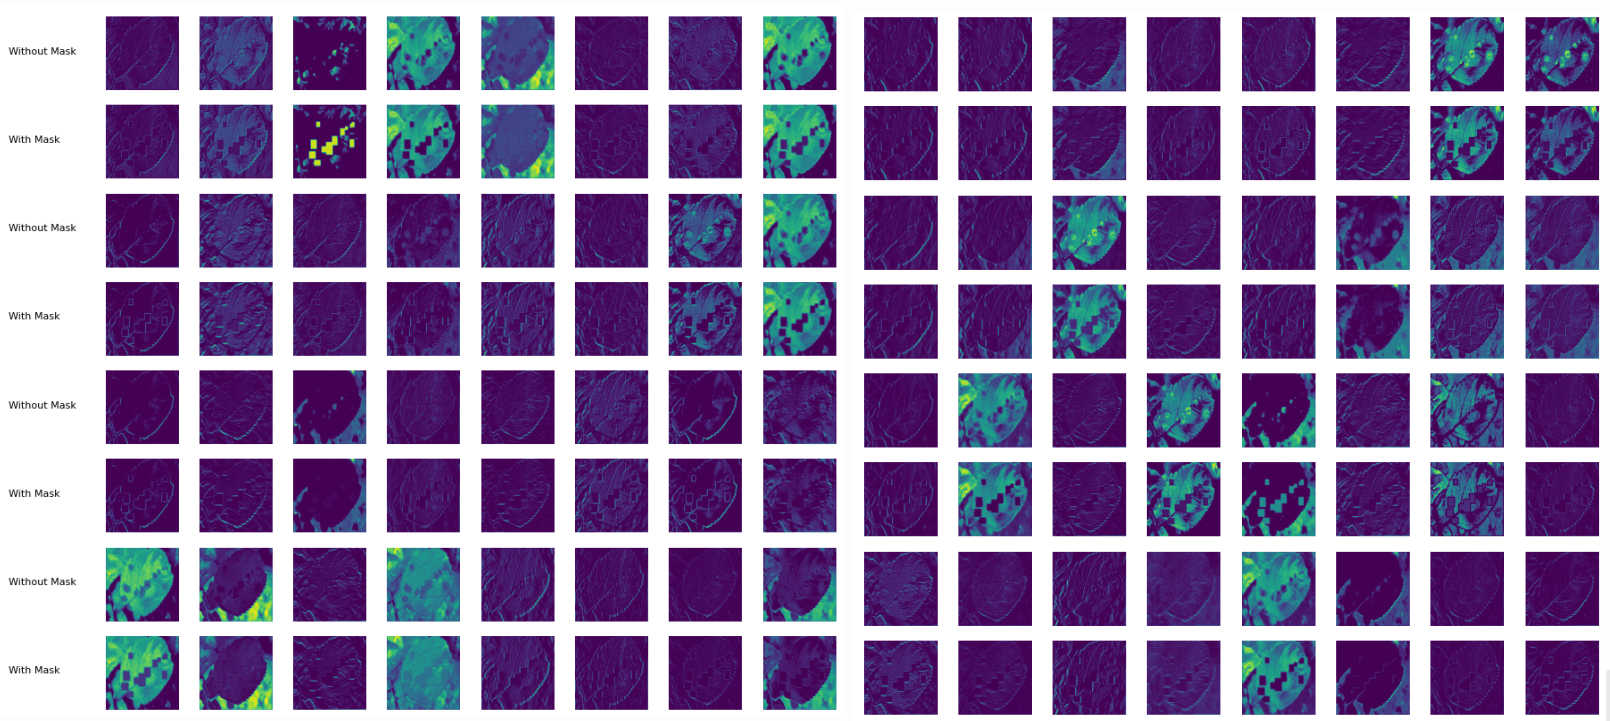
\includegraphics[width=1\linewidth]{graphics//chapter7/mask comparison l2.png}
         \caption{VGG16 base model Layer-2, first 64 Feature Map Comparison with Apple Scabs and Mask Apple Scabs}
        \label{fig:comp-1-1}
        \end{minipage}
    \end{turn}
\end{sidewaysfigure}


\begin{sidewaysfigure}
    \centering
    \begin{turn}{180}
        \begin{minipage}{\linewidth}
        \centering
        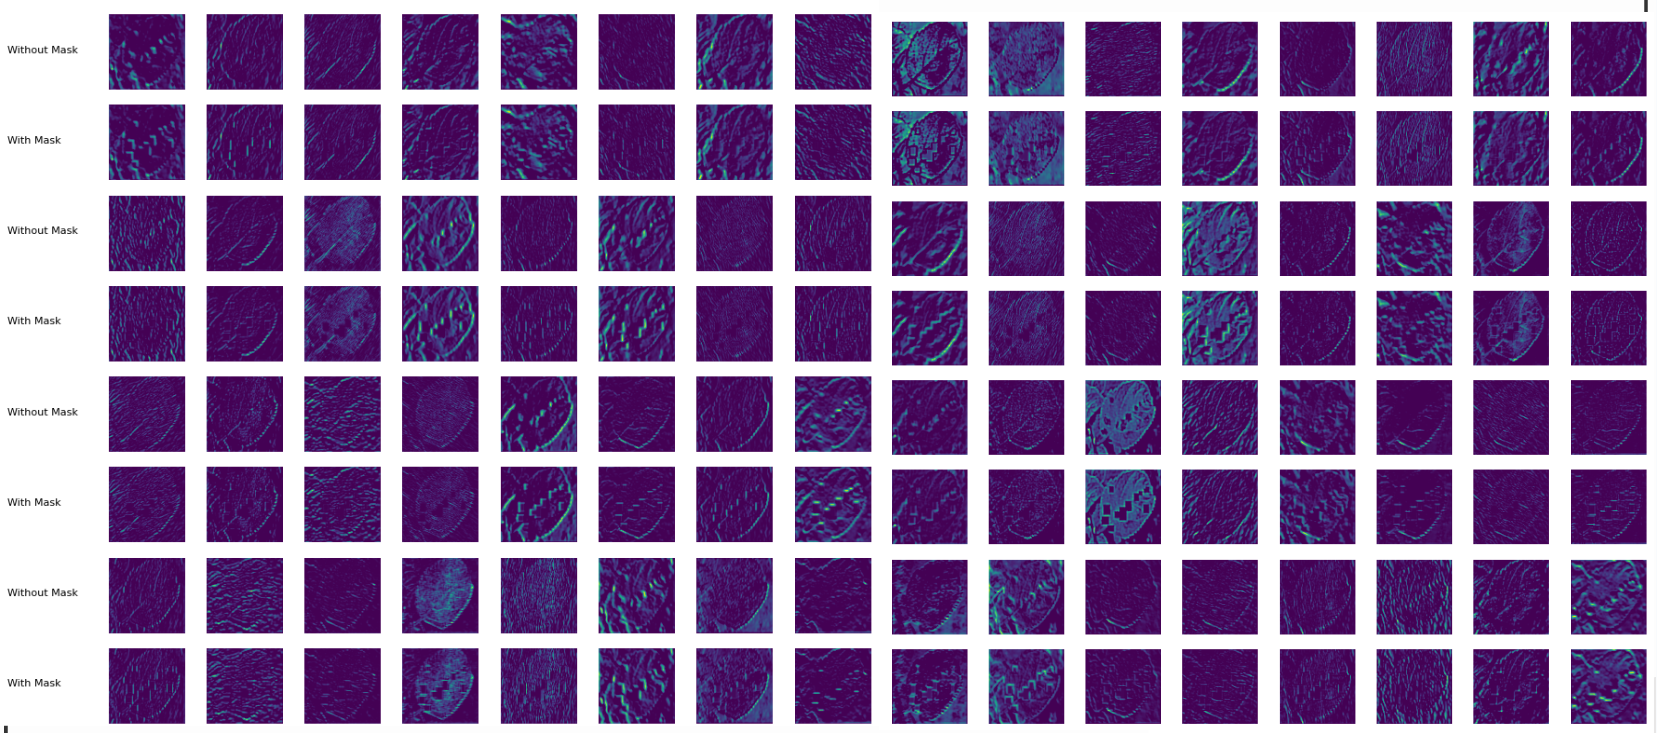
\includegraphics[width=1\linewidth]{graphics//chapter7/fmap comp mask l5.png}
        \caption{VGG16 base model Layer-5, first 64 Feature Map Comparison with Apple Scabs and Mask Apple Scabs}
    \label{fig:comp-1-2}
        \end{minipage}
    \end{turn}
\end{sidewaysfigure}

\begin{sidewaysfigure}
    \centering
    \begin{turn}{180}
        \begin{minipage}{\linewidth}
        \centering
        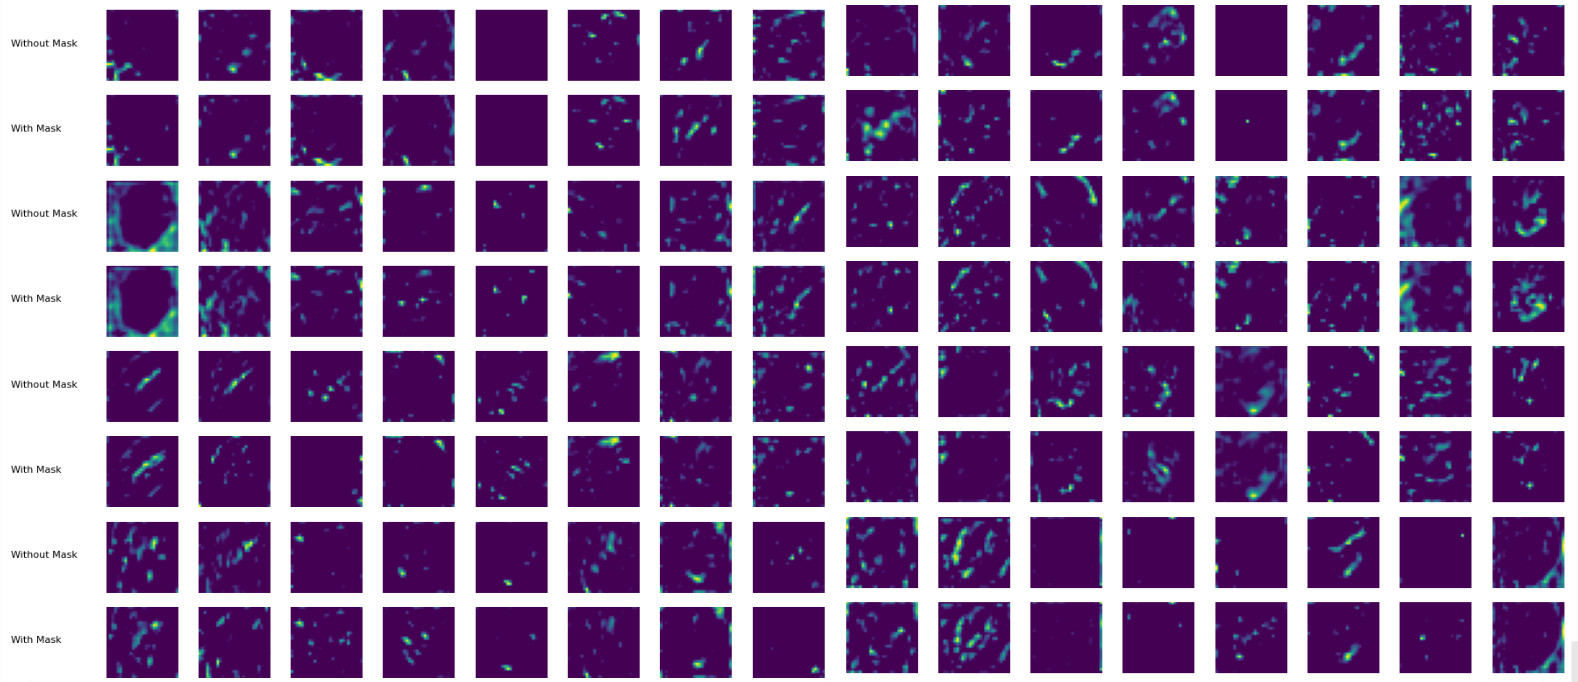
\includegraphics[width=1\linewidth]{graphics//chapter7/fmap comp mask l13.png}
         \caption{VGG16 base model Layer-13, first 64 Feature Map Comparison with Apple Scabs and Mask Apple Scabs}
         \label{fig:comp-1-3}
        \end{minipage}
    \end{turn}
\end{sidewaysfigure}

\begin{sidewaysfigure}
    \centering
    \begin{turn}{180}
        \begin{minipage}{\linewidth}
        \centering
        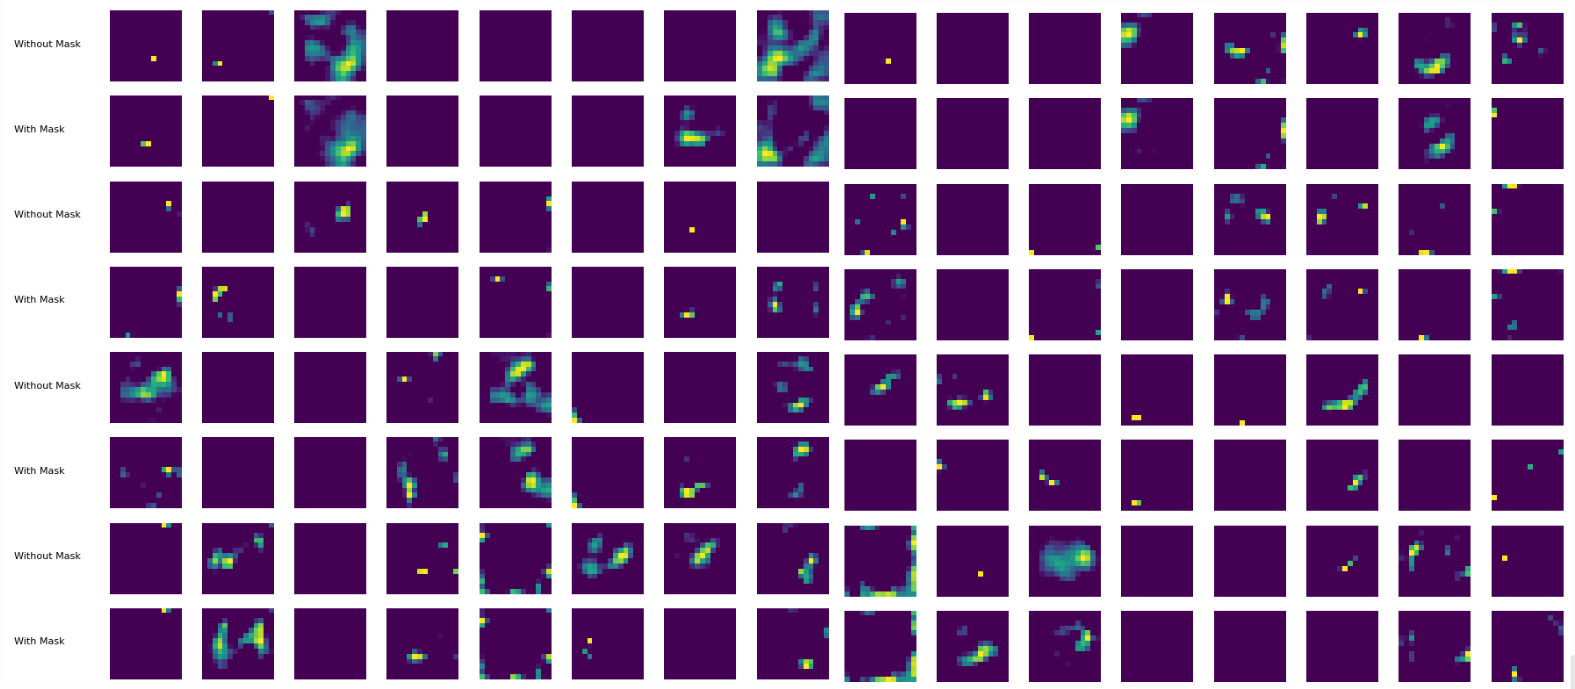
\includegraphics[width=1\linewidth]{graphics//chapter7/fmap comp mask l17.png}
         \caption{VGG16 base model Layer-17, first 64 Feature Map Comparison with Apple Scabs and Mask Apple Scabs}
    \label{fig:comp-1-4}
        \end{minipage}
    \end{turn}
\end{sidewaysfigure}

\textbf{Observation: }
\begin{itemize}
    \item \textbf{Normal Image: }\\
    When visualizing the feature maps of the normal image at various layers (2, 5, 9, 13, and 17), the model consistently captured detailed patterns, textures, and structures of the leaf. The feature maps showed strong activations corresponding to disease-specific areas, such as spots and discolorations, indicating that the model effectively identifies and processes relevant features for accurate classification.
    \item \textbf{Masked Image: }\\
    With the masked image, the feature maps at the same layers exhibited a notable reduction in activation in the masked region. However, the model still maintained strong activations in the unmasked areas. This suggests that while the mask affected the detection of features in the occluded region, the model was still able to extract and rely on the visible features to make informed predictions. This robustness highlights the model's ability to handle incomplete information and still focus on relevant, disease-specific characteristics present in the visible parts of the image.
\end{itemize}

   

\newpage
\section{Using PCA to vizualise Feature Space}
Principal component analysis (PCA) is a linear dimensionality reduction technique with applications in exploratory data analysis, visualization and data preprocessing.

The data is linearly transformed onto a new coordinate system such that the directions (principal components) capturing the largest variation in the data can be easily identified\cite{pca-0}\cite{pca-1}.

\subsection{Working of Principal Component Analysis (PCA)}
\begin{enumerate}
    \item \textbf{Standardize the Data}\\
    If the features of your dataset are on different scales, it’s essential to standardize them (subtract the mean and divide by the standard deviation).
    \item \textbf{Compute the Covariance Matrix}\\
        Calculate the covariance matrix for the standardized dataset. 
    \item \textbf{Compute Eigenvectors and Eigenvalues}\\
    Find the eigenvectors and eigenvalues of the covariance matrix. The eigenvectors represent the directions of maximum variance, and the corresponding eigenvalues indicate the magnitude of variance along those directions.
    \item \textbf{Sort Eigenvectors by Eigenvalues}\\
    Sort the eigenvectors based on their corresponding eigenvalues in descending order.
    \item \textbf{Choose Principal Components}\\
    Select the top k eigenvectors (principal components) where k is the desired dimensionality of the reduced dataset.
    \item \textbf{Transform the Data}\\
    Multiply the original standardized data by the selected principal components to obtain the new, lower-dimensional representation of the data.\cite{pca-1}
\end{enumerate}

\subsection{PCA Feature Space Visualisation}
To analyze the feature representation learned by our models, we visualized the feature space using Principal Component Analysis (PCA). This analysis helps in understanding how well the model distinguishes between different classes based on the extracted features.\par\vspace{1em}

\subsection{Before Fine Tuning}

\begin{figure}
    \centering
    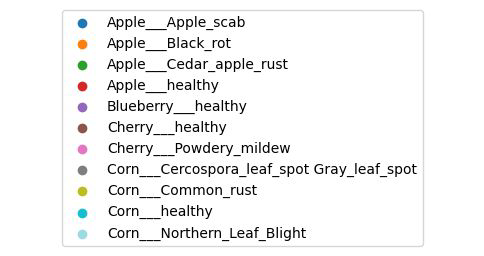
\includegraphics[width=0.5\linewidth]{graphics//chapter7/pca legend.png}
    \caption{Legend used in feature space vizualization}
    \label{fig:pca-legend}
    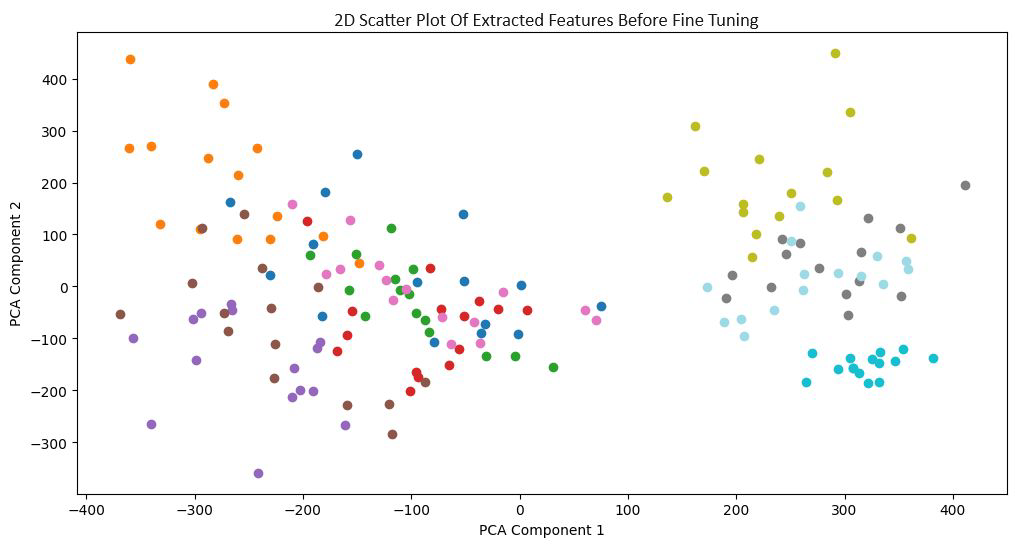
\includegraphics[width=1\linewidth]{graphics//chapter7/pca viz bft 2d.png}
    \caption{VGG16 Feature Space Visualisation Before Fine Tuning Using PCA in 2D}
    \label{fig:pca-bft-2d}
    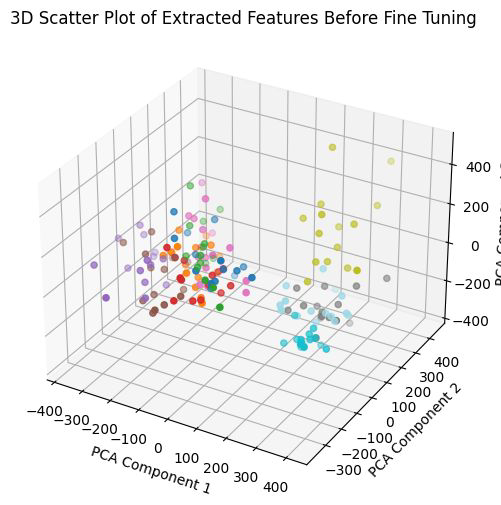
\includegraphics[width=0.65\linewidth]{graphics//chapter7/pca viz bft 3d.png}
    \caption{VGG16 Feature Space Visualisation Before Fine Tuning Using PCA in 3D}
    \label{fig:pca-bft-3d}
\end{figure}

\textbf{Observations}: refer fig\ref{fig:pca-bft-2d}
\begin{itemize}
    \item When applying PCA to the features extracted by the pre-trained VGG16 model, the visualization did not show distinct clusters. Images from different classes were intermixed, indicating that the features were not sufficiently discriminative for different plant diseases.
    \item Leaves from the same species, regardless of disease, were often grouped together. This suggests that the pre-trained model's features were more influenced by species characteristics rather than disease-specific traits.
\end{itemize}

\subsection{After Fine Tuning}

\begin{figure}
    \centering
    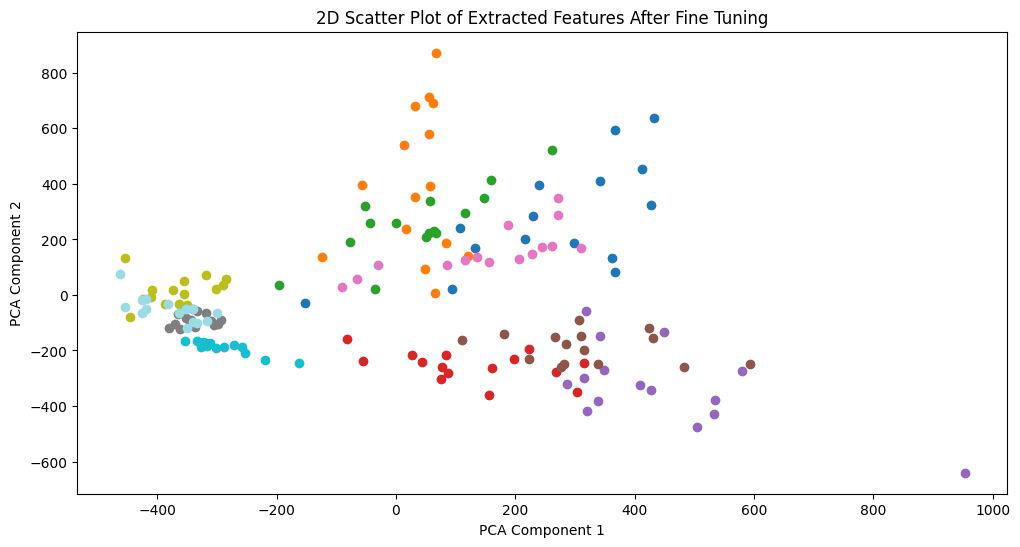
\includegraphics[width=1\linewidth]{graphics//chapter7/pca vis aft 2d.png}
    \caption{VGG16 Feature Space Visualisation After Fine Tuning using PCA in 2D}
    \label{fig:pca-aft-2d}
    
    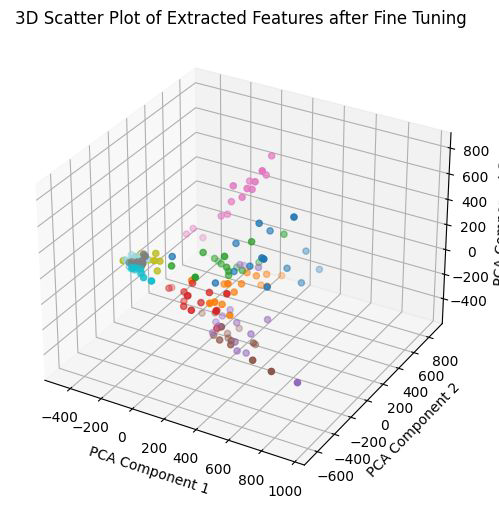
\includegraphics[width=0.75\linewidth]{graphics//chapter7/pca vis after fine tuning 3d.png}
    \caption{Feature Space Visualisation After Fine Tuning using PCA on 3D}
    \label{fig:pca-aft-}
\end{figure}

\textbf{Observations}: \ref{fig:pca-aft-2d}
\begin{itemize}
    \item After fine-tuning the VGG16 model on the Plant Village dataset, the PCA visualization showed somewhat clearer clusters. There was a noticeable improvement in the separation of different disease classes, although the clusters were still not very distinct.
\end{itemize}

\FloatBarrier

\section{Using t-SNE to vizualise Feature Space}
t-distributed stochastic neighbor embedding (t-SNE) is a statistical method for visualizing high-dimensional data by giving each datapoint a location in a two or three-dimensional map.
It is a nonlinear dimensionality reduction technique for embedding high-dimensional data for visualization in a low-dimensional space of two or three dimensions\cite{tsne-0}\cite{tsne-1}\cite{tsne-2}.\par\vspace{1em}

Since, feature space visualisation using PCA, doesn't provide work as expected by our team, we perform the same visualisation technique using t-SNE and get our expected results in the feature space visualisation both in 2D and 3D features space.

\subsection{Before Fine Tuning}

\begin{figure}
    \centering
    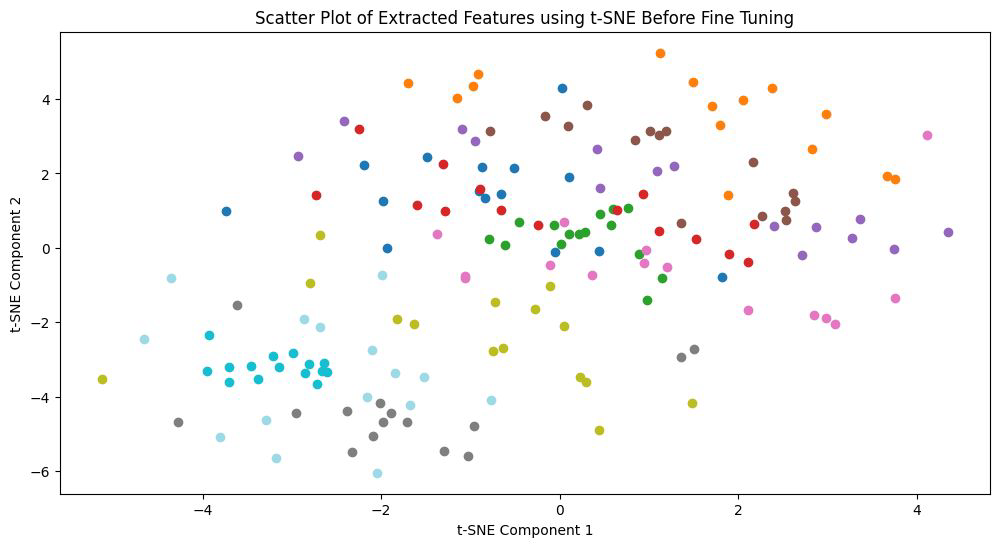
\includegraphics[width=1\linewidth]{graphics//chapter7/vgg feature viz tsne 2d.png}
    \caption{VGG16 Feature Space Visualisation Before Fine Tuning using t-SNE in 2D}
    \label{fig:tsne-bft-2d}
\end{figure}
\begin{figure}
    \centering
    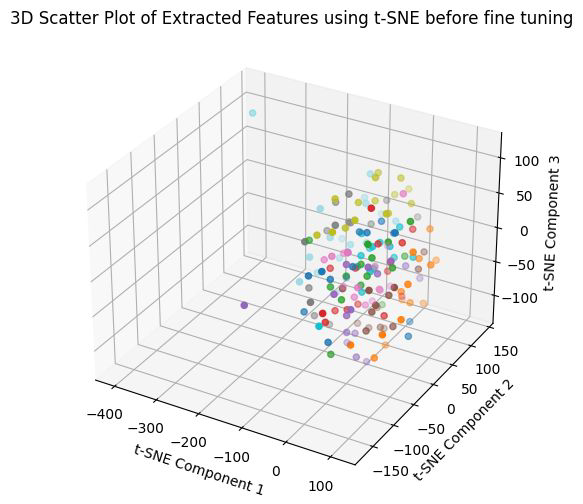
\includegraphics[width=0.75\linewidth]{graphics//chapter7/vgg feature vuz tsne before fine tuning 3d.png}
    \caption{VGG16 Feature Space Visualisation Before Fine Tuning using t-SNE in 3D}
    \label{fig:tsne-bft-3d}
\end{figure}
\textbf{Observations: } refer fig\ref{fig:tsne-bft-2d}
\begin{itemize}
    \item Using t-SNE on the same features also resulted in poorly defined clusters. The intermixing of different disease classes persisted, further confirming that the pre-trained model did not adequately separate the disease classes in the feature space.
\end{itemize}

\subsection{After Fine Tuning}
\begin{figure}
    \centering
    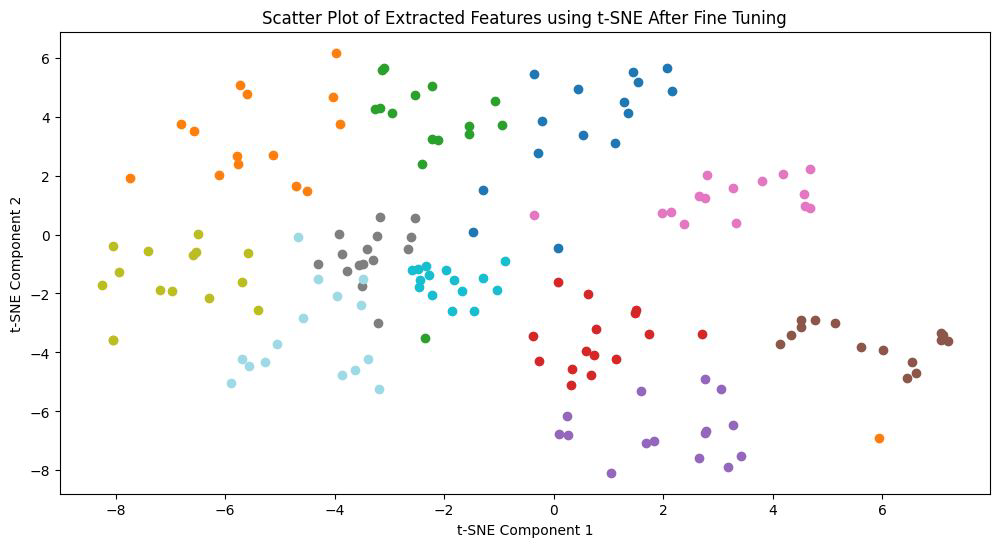
\includegraphics[width=1\linewidth]{graphics//chapter7/vgg feature viz after fine tuning 2d.png}
    \caption{VGG16 Feature Space Visualisation After Fine Tuning using t-SNE in 2D}
    \label{fig:tsne-aft-2d}
\end{figure}

\begin{figure}
    \centering
    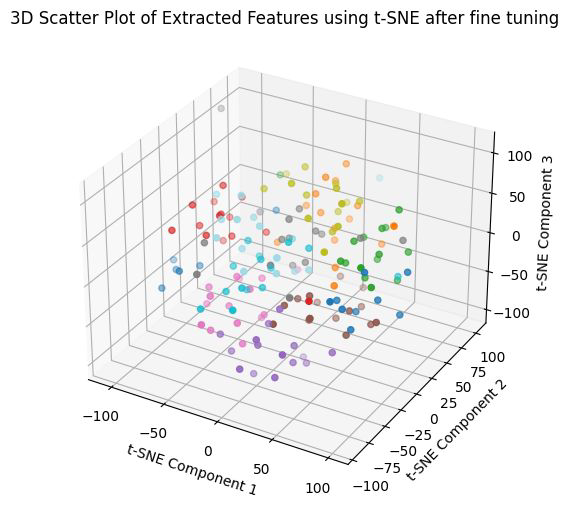
\includegraphics[width=0.75\linewidth]{graphics//chapter7/vgg feature viz after fine tuning tsne.png}
    \caption{VGG16 Feature Space Visualisation After Fine Tuning using t-SNE in 3D}
    \label{fig:tsne-aft-3d}
\end{figure}
\textbf{Observations: } fig\ref{fig:tsne-aft-2d}
\begin{itemize}
    \item Applying t-SNE to the features from the fine-tuned VGG16 model revealed prominent clusters for each class. The visualization showed that the fine-tuned model could effectively separate different disease classes, with each class forming its own local cluster.
    \item Unlike the pre-tuned model, the fine-tuned model’s feature space demonstrated that leaves were clustered based on disease classes rather than species. Leaves of the same species but different diseases were now separated, indicating that the fine-tuned model learned disease-specific features.
\end{itemize}


\fbox{
    \parbox{\textwidth}{
        The feature space visualization using PCA and t-SNE highlights the significant improvements achieved through fine-tuning. Before fine-tuning, the pre-trained model's features were not adequately distinguishing between different diseases, often clustering images based on species. After fine-tuning, the model learned more discriminative features, leading to clearer separation of disease classes in the feature space, by forming local cluster and also preserving the information that these images are from the same species as the local cluster of each plant disease from the same plant disease are located closely in the feature space.  \par\vspace{1em}
        For example, this fig \ref{fig:pca-aft-2d}, we observe that the fine tuned VGG16 base model group \textit{Corn} plant species together globally in the feature space and also we observe that individual corn disease are also clustered together locally.  \par\vspace{1em}
        This enhanced representation underscores the effectiveness of fine-tuning in adapting pre-trained models to specific classification tasks, resulting in more accurate and reliable predictions.\par\vspace{1em}
    }
}



\FloatBarrier
\newpage
\section{Visualising Nearest Neighbors in Features Space}


In this technique, we used Cosine similarity,\\

\[\mathit{cosineSimilarity(A, B)} = cos(\theta) = \frac{A * B}{|A| * |B|}\]
 \\
to find and visualize the nearest neighbors of a query image in the feature space. The features from our image is extracted using our fine tuned VGG16 base model.\par\vspace{1em}  From analysis of nearest neighbor using cosine similarity, we observe that the nearest neighbors data instance in feature space exhibits similar features to the query image. These demonstrate the model's ability to group similar images effectively\par\vspace{1em}

The steps we take to perform in this technique are as follows:\par\vspace{1em}
\begin{algorithm}
\caption{Find Nearest Neighbors in Feature Space}
\label{alg:nearest_neighbors}

\textbf{Input:}
\begin{itemize}
    \item \textit{query\_image}: Image for which nearest neighbors are to be found
    \item \textit{Feature Extractor}: Pretrained model to extract features
    \item \textit{Image Dataset}: Dataset containing images
    \item \textit{N}: Number of nearest neighbors to find
\end{itemize}

\textbf{Output:}
\begin{itemize}
    \item \textit{Nearest neighbors}: List of N nearest images to the query image in feature space
\end{itemize}

\begin{algorithmic}[1]
    \State Extract feature from the \textit{query image} using the \textit{feature extractor} model
    \State Similarly, extract features from all image in image dataset
    \State Compute cosine similarity with query image features and all other image features
    \State From the cosine similarity result find the \textbf{\textit{N}} largest value and plot the corresponding image on graph
\end{algorithmic}
\end{algorithm}


\subsection{Before Fine Tuning}
\begin{figure}
    \centering
    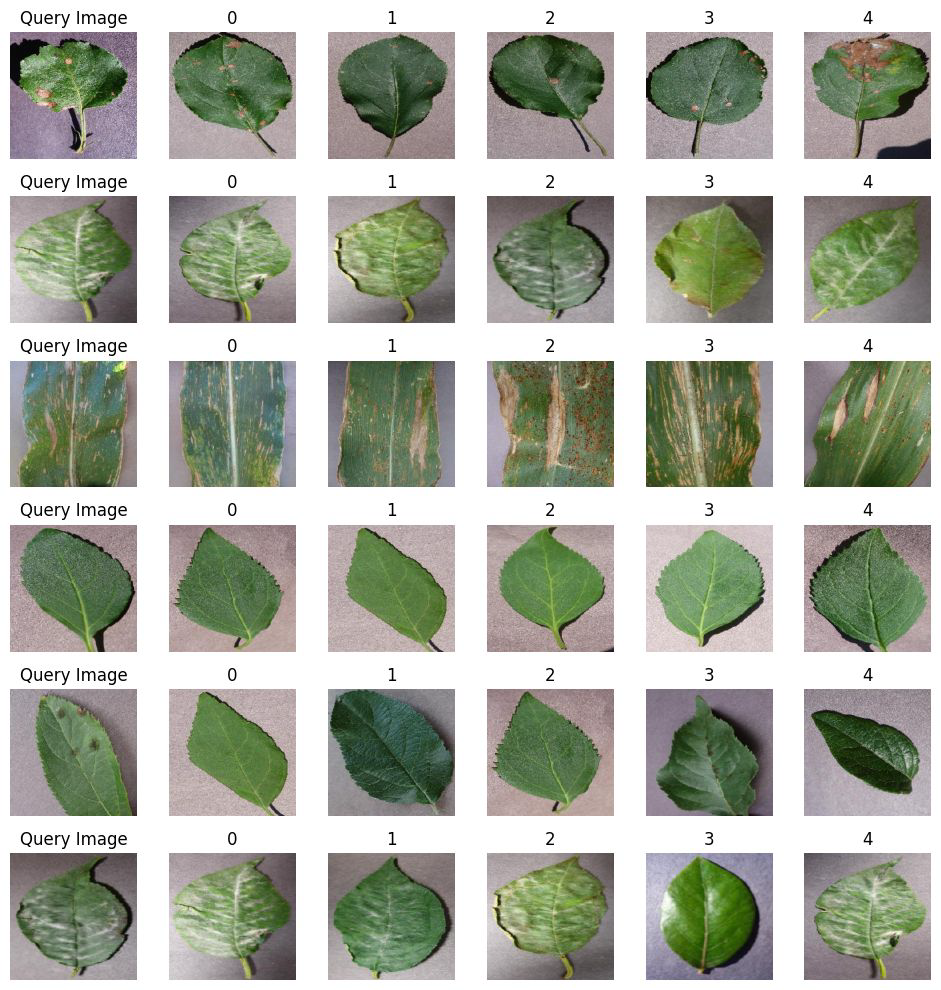
\includegraphics[width=1\linewidth]{graphics//chapter7/query image bft.png}
    \caption{Feature Space Nearest Neighbour Before Fine Tuning, where image labeled 0 in each row is the closest to the query image in feature space and labeled 1 is the second closest and so on.}
    \label{fig:query-bft}
\end{figure}

In this phase we, observe the following:
\begin{itemize}
    \item When querying the pre-trained VGG16 model with an image of apple black rot, the nearest neighbors included images of healthy apple leaves, apple scab, and other apple diseases.
    \item This indicates that the feature representations learned from the ImageNet dataset were not sufficiently specialized to distinguish between different types of apple diseases. The model grouped various apple-related images closely, despite differences in disease characteristics.
\end{itemize}

\subsection{After Fine Tuning}
\begin{figure}
    \centering
    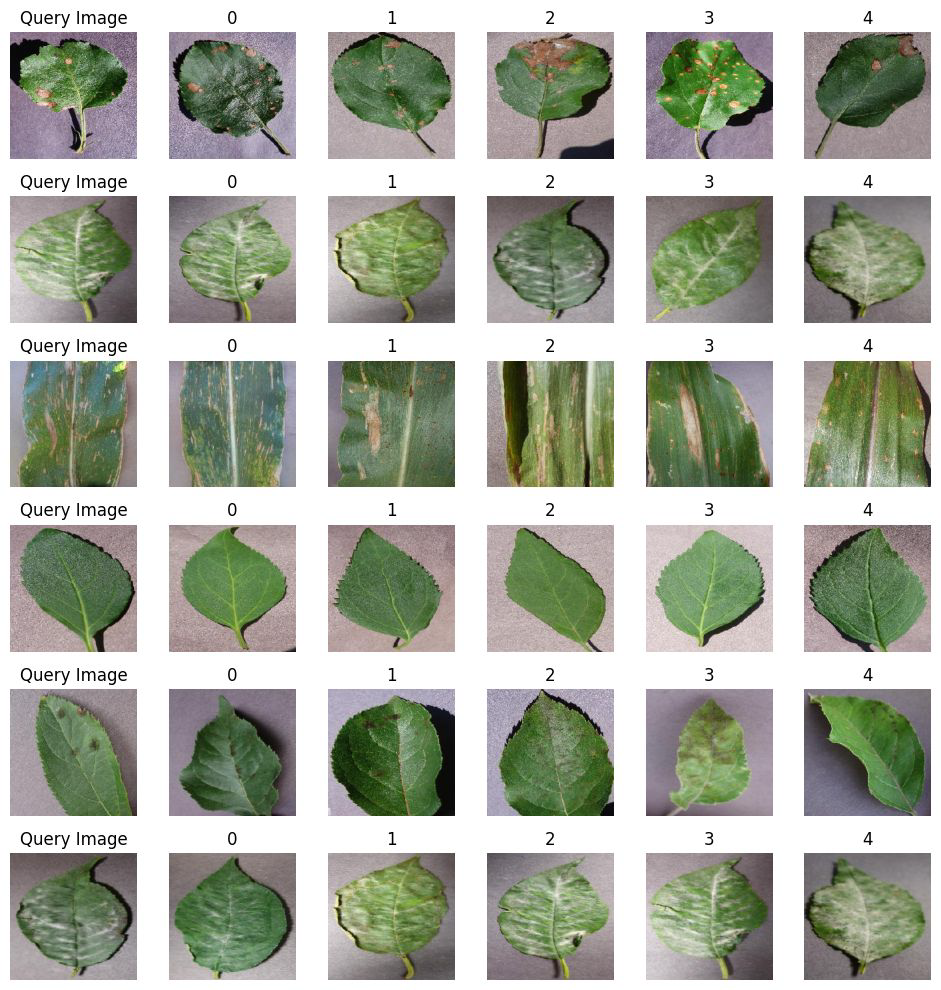
\includegraphics[width=1\linewidth]{graphics//chapter7/query after fine tuning.png}
    \caption{Feature Space Nearest Neighbors After Fine Tuning, where image labeled 0 in each row is the closest to the query image in feature space and labeled 1 is the second closest and so on.}
    \label{fig:query-aft}
\end{figure}
After Fine Tuning our model, we, observe that:
\begin{itemize}
    \item After fine-tuning the VGG16 model on the Plant Village dataset, the nearest neighbor results showed a significant improvement.
    \item When the same query image of apple black rot was used, the nearest neighbors identified by the model were predominantly images of apple black rot, demonstrating a high degree of specificity.
    \item This improvement suggests that fine-tuning allowed the VGG16 model to learn more precise and relevant features specific to the Plant Village dataset, enhancing its ability to correctly differentiate between similar classes.
\end{itemize}

The nearest neighbor analysis highlights the effectiveness of fine-tuning in improving model performance. By adapting the pre-trained weights to the specific characteristics of plant disease images, the fine-tuned VGG16 model achieved a better representation of disease-specific features, leading to more accurate and reliable classifications.\par\vspace{1em}

\FloatBarrier

\newpage
\section{Saliency Maps}

In computer vision, a saliency map is an image that highlights either the region on which people's eyes focus first or the most relevant regions for machine learning models. The goal of a saliency map is to reflect the degree of importance of a pixel to the human visual system or an otherwise opaque ML model\cite{smap-paper}\cite{smap-paper-1}.\par \vspace{1em}

\fbox{
    \parbox{\textwidth}{
        A saliency map highlights the important parts of an image that a machine learning model focuses on when making a prediction. It shows which pixels in the image have the most influence on the model's decision.
    }
}

\subsection{Explainable Artificial Intelligence using Saliency Map}

Explainable Artificial Intelligence in the context of black box machine learning models: Saliency maps are a prominent tool providing visual explanations of the decision-making process of machine learning models, particularly deep neural networks. These maps highlight the regions in input images, text, or other types of data that are most influential in the model's output, effectively indicating where the model is "looking" when making a prediction. By illustrating which parts of the input are deemed important, saliency maps help in understanding the internal workings of otherwise black box models, thereby fostering trust and transparency. In image classification tasks, for example, saliency maps can identify pixels or regions that contribute most to a specific class decision. One of the most prominent techniques to generate saliency maps is Gradient-weighted Class Activation Mapping (Grad-CAM).

\subsection{Steps for Generating Saliency Maps}
The steps are as follows: 
\begin{enumerate}
    \item Prediction:\\
    First, we pass an input image through the model to get its prediction. The model outputs a set of scores (or probabilities) for each possible class. For example, if the model is a dog breed classifier, it might output scores for classes like "Labrador", "Poodle", "Bulldog", etc.
    
    \item Identify the Top Class:\\
    We identify the class with the highest score. This is the class that the model thinks the image most likely belongs to. Let's call this the "top class."
    
    \item Compute the Gradient:\\
    To understand which parts of the image contributed most to the top class score, we compute the gradient of this score with respect to each pixel in the input image.\\
    The gradient tells us how much a small change in each pixel would affect the top class score. If changing a pixel significantly increases the score, that pixel is important for the model's prediction.
    
    \item Take the Absolute Value:
    We take the absolute value of these gradients. This step is important because we care about the magnitude of the impact (how much it affects the score) rather than the direction (whether it increases or decreases the score).
    
    \item Aggregate Across Color Channels:\\
    If the image has multiple color channels (like RGB), we combine the gradients across these channels. A common approach is to take the maximum gradient value across the channels for each pixel. This gives us a single importance value per pixel.
    
    \item Create the Saliency Map:\\
    The result is a saliency map, where each pixel's value represents its importance in the model's prediction. High values indicate pixels that had a strong influence on the top class score, while low values indicate less important pixels.
    
\end{enumerate}
\par\vspace{1em}

\begin{figure}
    \centering
    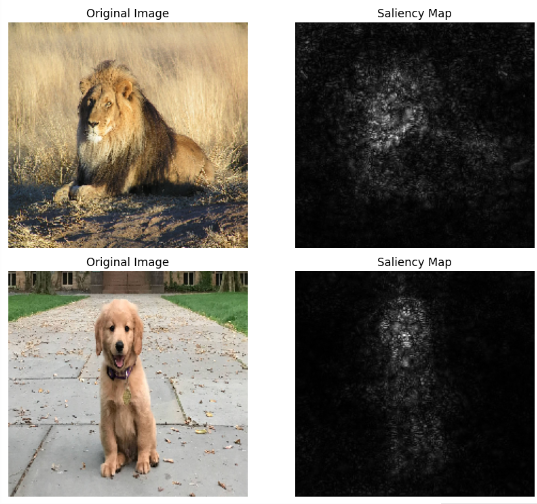
\includegraphics[width=1\linewidth]{graphics//chapter7/smap vgg160.png}
    \caption{Saliency Map Generated by VGG16 trained on ImageNet }
    \label{fig:smap-0}
\end{figure}

The key idea behind saliency maps is using gradients, which are a core concept in how neural networks learn. During training, gradients show how to adjust weights to reduce the error. Here, we use gradients to see how changes in the input image affect the model's output, highlighting the parts of the image that are most influential.\cite{smap-paper}\cite{WEBSITE:smap-ref}
\par\vspace{1em}


\begin{figure}
    \centering
    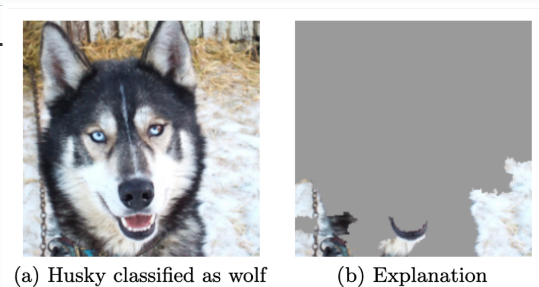
\includegraphics[width=1\linewidth]{graphics//chapter7/smap dog breed.png}
    \caption{Saliency Map Generated by a Dog Classifier Model}
    \label{fig:smap-1}
\end{figure}

\begin{figure}
    \centering
    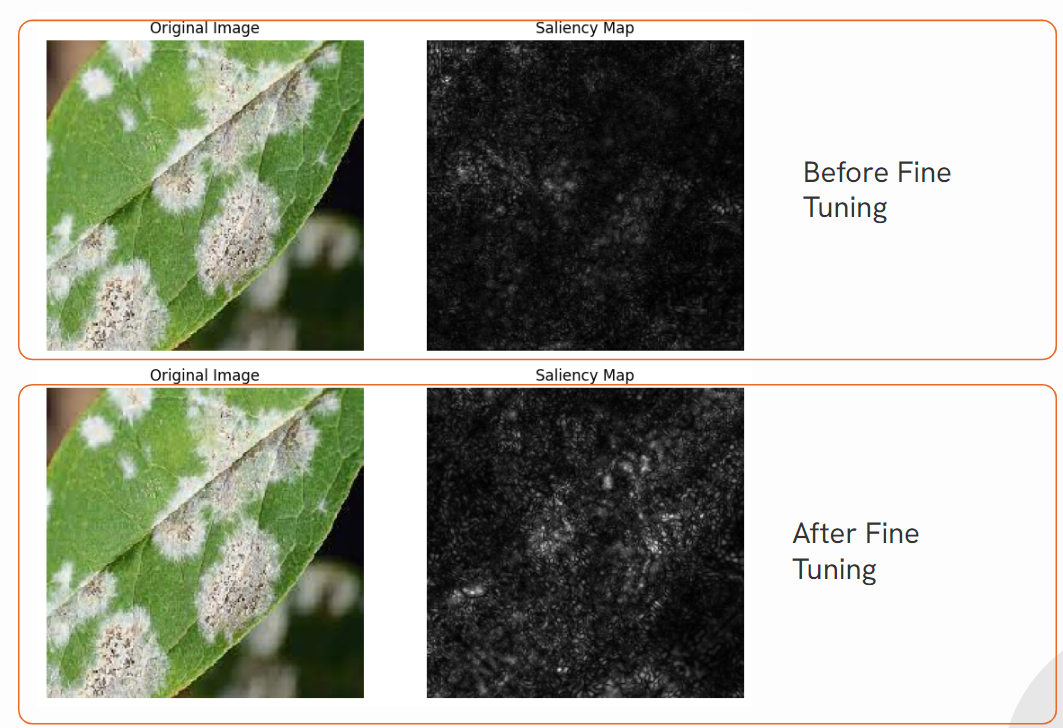
\includegraphics[width=1\linewidth]{graphics//chapter7/vgg smap1.png}
    \caption{Saliency Map Generated by VGG16 base model before and after Fine Tuning on Plant Village Datasets}
    \label{fig:smap-2}
\end{figure}


\begin{figure}
    \centering
    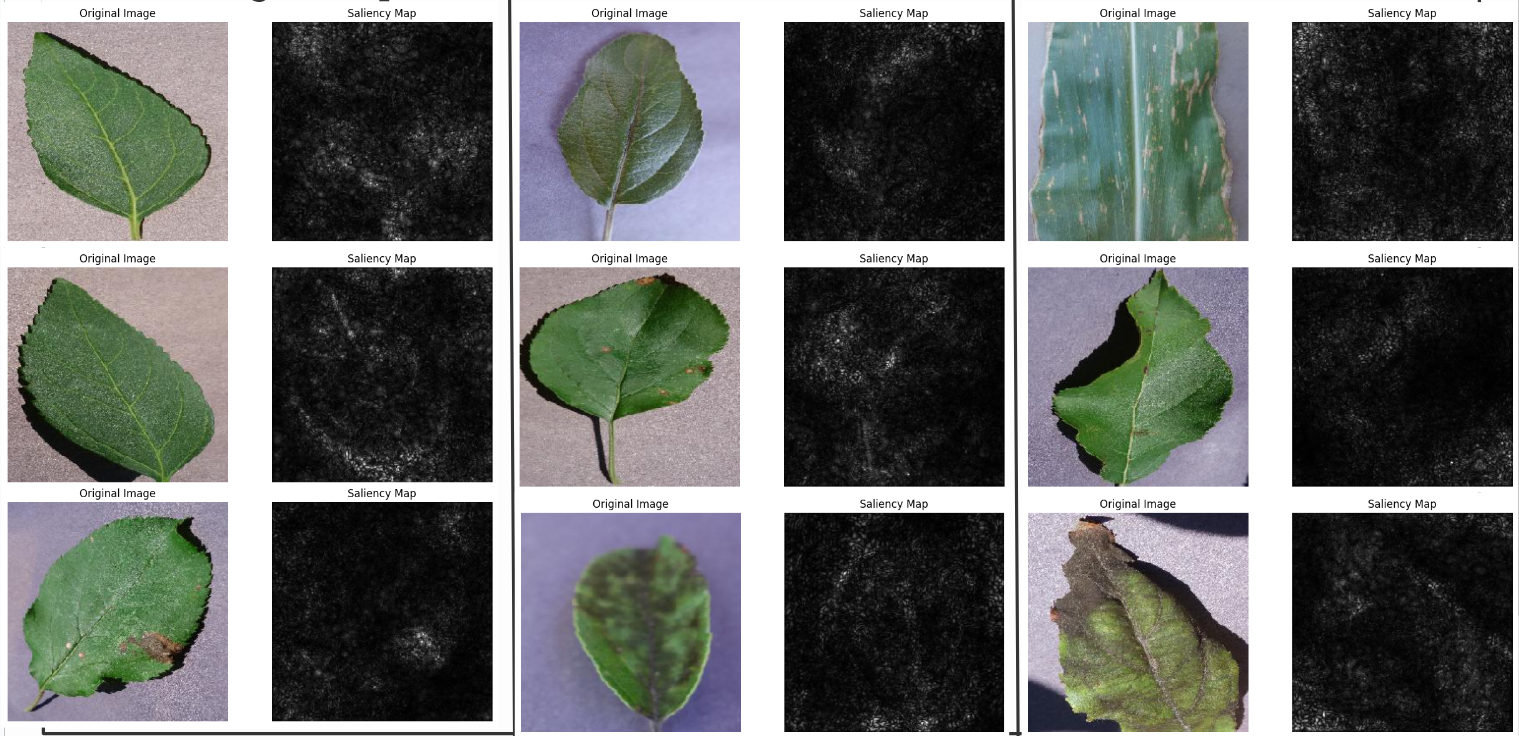
\includegraphics[width=1\textheight, angle=90, origin=c]{graphics//chapter7/vgg smap2.png}
    \caption{Saliency Map generated by VGG16 base model before fine tuning}
    \label{fig:smap-3}
\end{figure}


% \begin{figure}[h]
%     \centering
%     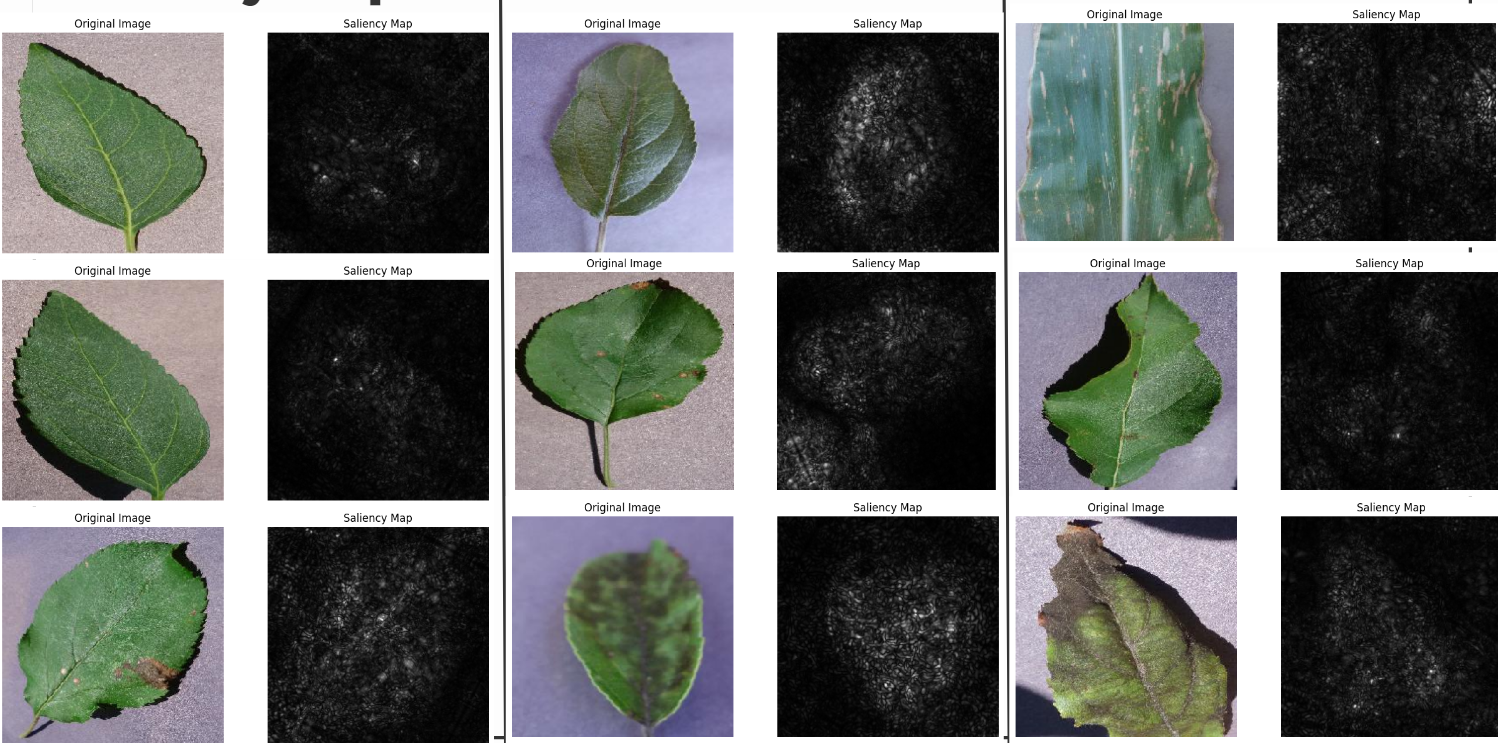
\includegraphics[width=1\textheight, angle=90, origin=c]{graphics//chapter7/vgg smap 3.png}
%     \caption{Saliency Map generated by VGG16 base model after fine tuning last}
%     \label{fig:smap-4}
% \end{figure}



\begin{figure}[h]
    \centering
    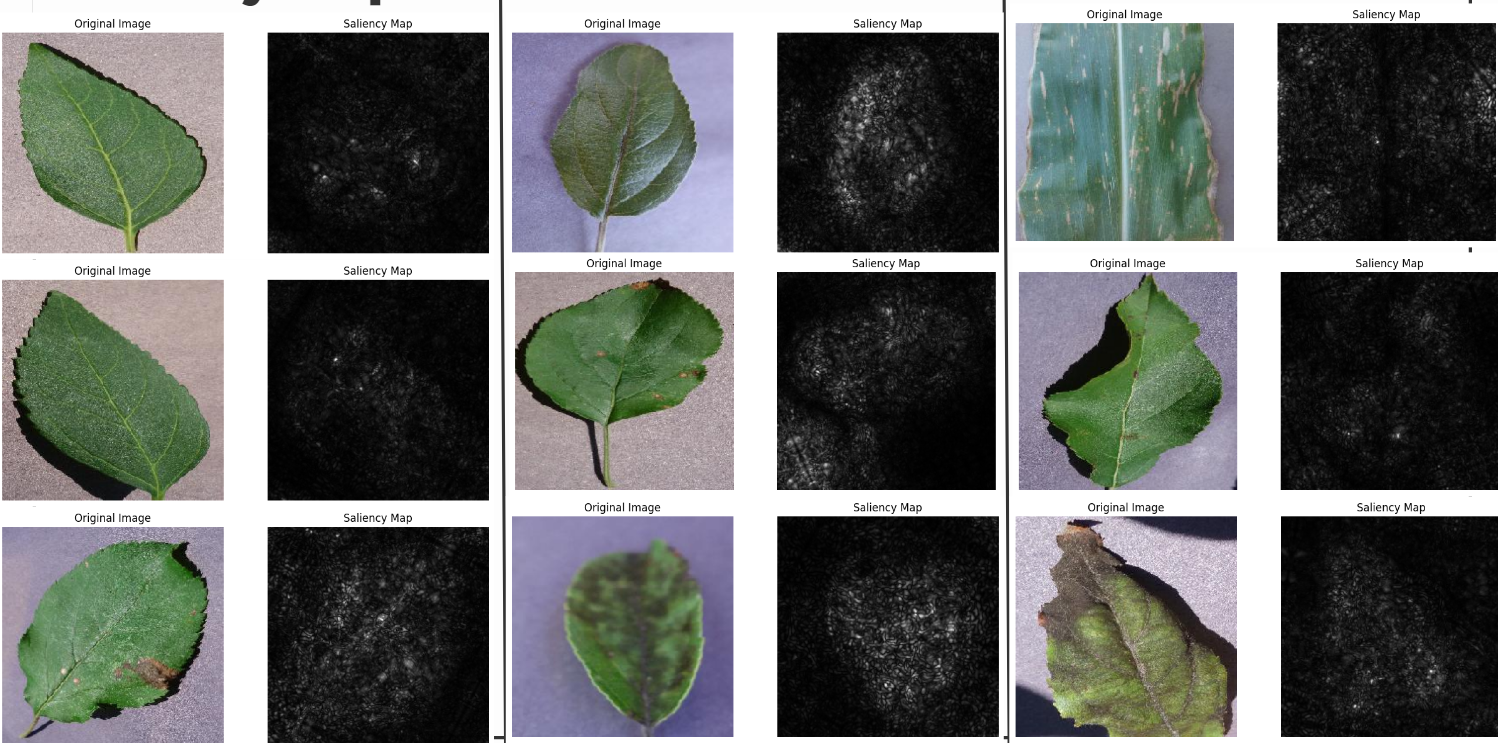
\includegraphics[width=1\textheight, angle=90, origin=c]{graphics//chapter7/vgg smap 3.png}
    \caption{Saliency Map generated by VGG16 base model after fine tuning last}
    \label{fig:smap-4}
\end{figure}
\subsection{Observations from Saliency Map}

In our observations of saliency maps generated by both a pre-trained model and a fine-tuned model, several notable differences emerges. The pretrained model is effectively good in highlighting regions of images which are of general interest in classification tasks, fig: \ref{fig:smap-0}, but in specialized task it produces broader and less precise saliency regions. This is likely due to its training on a generalized training datasets, which help them to equip with a wide-ranging but somewhat superficial understanding of features.\par\vspace{1em}
In contrast, the fine-tuned model demonstrates a marked improvement in the specificity and relevancy of the saliency map. Fine tuning the model on plant village datasets allows it to adapt and improve its feature detection capabilities, resulting in more accurate and focused identification of critical regions of the image.\par\vspace{1em}
For example: in fig:\ref{fig:smap-2}\, we observe that before fine-tuning our models does not have a clear ideas on which areas to focus, but after fine tuning, we observe that the model tries to focus on the regions of leaves which are affected (white spot regions).
\par\vspace{1em}
In fig: \ref{fig:smap-3} and fig:\ref{fig:smap-4}, we provide another visualization of saliency map produced by our model, before and after fine tuning on 9 data instances. Some of the observation that are notable ones is 3-row, 2-col image, we observe that the model focus on the whole regions of images, even the background, but after fine tuning, it focus only on  the infected region of the leaves.
\FloatBarrier